\chapter{驾驶人行为特性的差异性分析}
本章的研究目的在于探究驾驶人行为特性,在专业与非专业驾驶人中是否存在差异,在哪些方面存在差异以及差异的程度有多大,为下一章研究驾驶人行为特性对交通流影响提供依据。本章首先将讨论所获取数据的基本情况,针对数据所存在的问题进行数据后处理。其次,对数据进行集计,分析两组受试驾驶人在跟驰行为中所表现出的特性。最后,使用测试数据对跟驰模型参数进行标定,并分析两组驾驶人参数分布的异同。
\section{数据处理}
\subsection{数据基本情况}
\subsubsection{驾驶人构成}

根据第三章对于驾驶人分类,区别专业与非专业驾驶人的主要因素为驾龄,总里程数。专业驾驶人主要选取长期从事驾驶工作,驾龄7年以上且累计行程10万公里以上的驾驶人;非专业驾驶人主要选取非特定职业,驾龄不足7年或累计行程不足10万公里的驾驶人。

应征驾驶人共26人,其中10人归为非专业驾驶人16人归为专业驾驶人,其基本情况如下,驾驶人的年龄分布如\autoref{age_barplot},其中最大的群体为20-25岁。两组驾驶人的年龄分布箱图如\autoref{age_boxplot},其中专业驾驶人平均年龄为43.4岁,最低33岁,最高53岁;非专业驾驶人专业驾驶人平均年龄为25岁,最低23岁,最高29岁。

两组驾驶人的驾龄和累计行驶里程分布情况分别如\autoref{certified_boxplot}和\autoref{mileage_boxplot},实验样本中,非专业组平均驾龄为3.06年,平均行驶里程为2.01万公里专业组平均驾龄为12.6年,平均行驶里程为67.2万公里。

可以看出非专业组和专业组驾驶人的驾龄和累计行驶里程存在明显的差异,但是驾驶人的驾龄、累计行驶里程和年龄似乎存在较大的相关性。

另外值得一提的是实验样本中的女性驾驶人较少仅有3名,占样本量26名的约10\%,3名女性驾驶人均为非专业驾驶人。



\begin{figure}
\begin{minipage}[t]{0.48\linewidth}
\centering
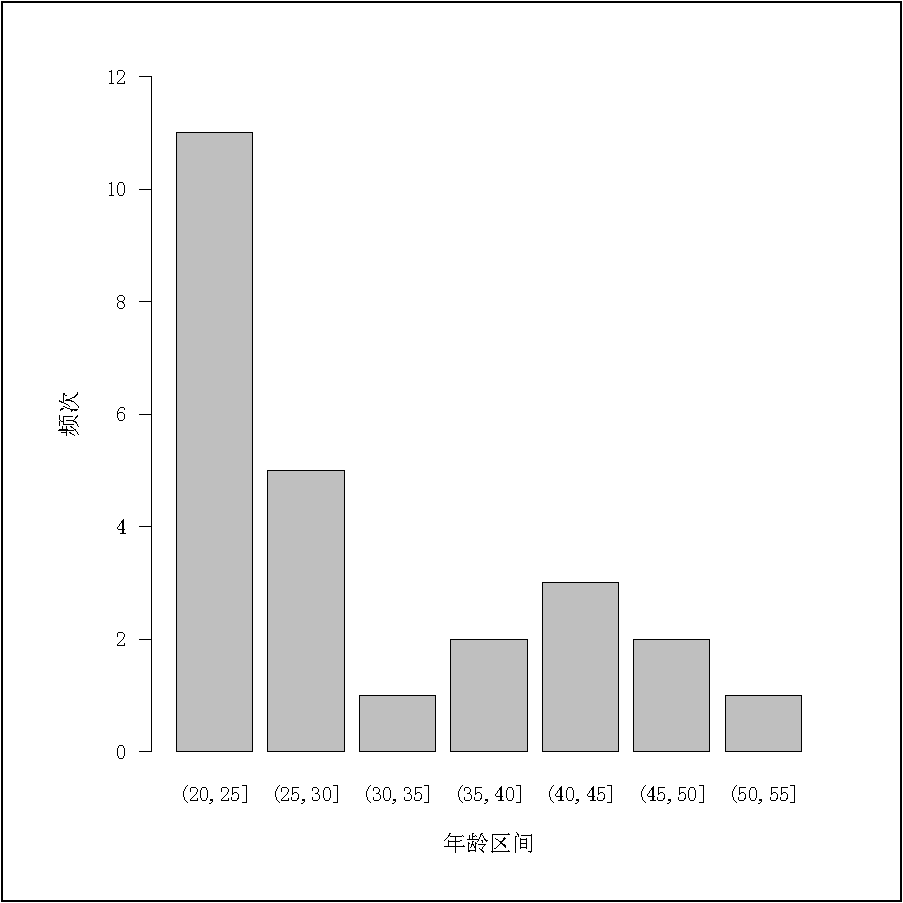
\includegraphics[width=\textwidth]{chapter4-age_barplot}
\caption{年龄分布柱状图}
\label{age_barplot}
\end{minipage}%
\hspace*{0.04\linewidth}
\begin{minipage}[t]{0.48\linewidth}
\centering
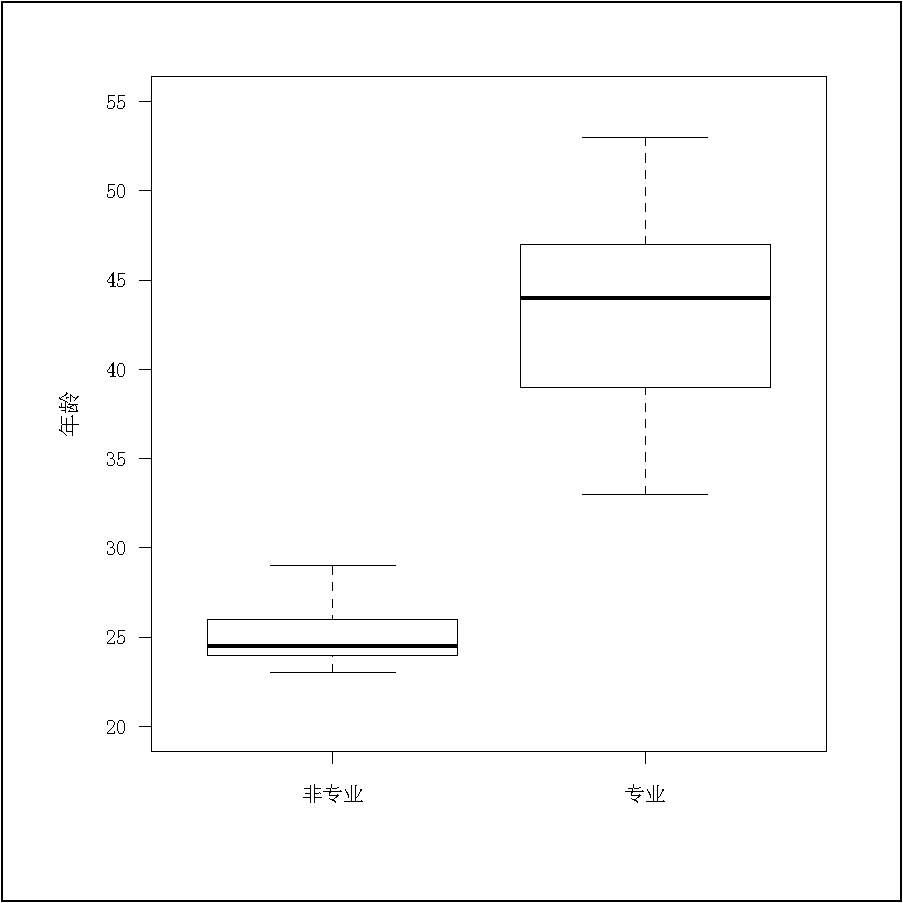
\includegraphics[width=\textwidth]{chapter4-age_boxplot}
\caption{非专业与专业组年龄箱图}
\label{age_boxplot}
\end{minipage}
\end{figure}

\begin{figure}
\begin{minipage}[t]{0.48\linewidth}
\centering
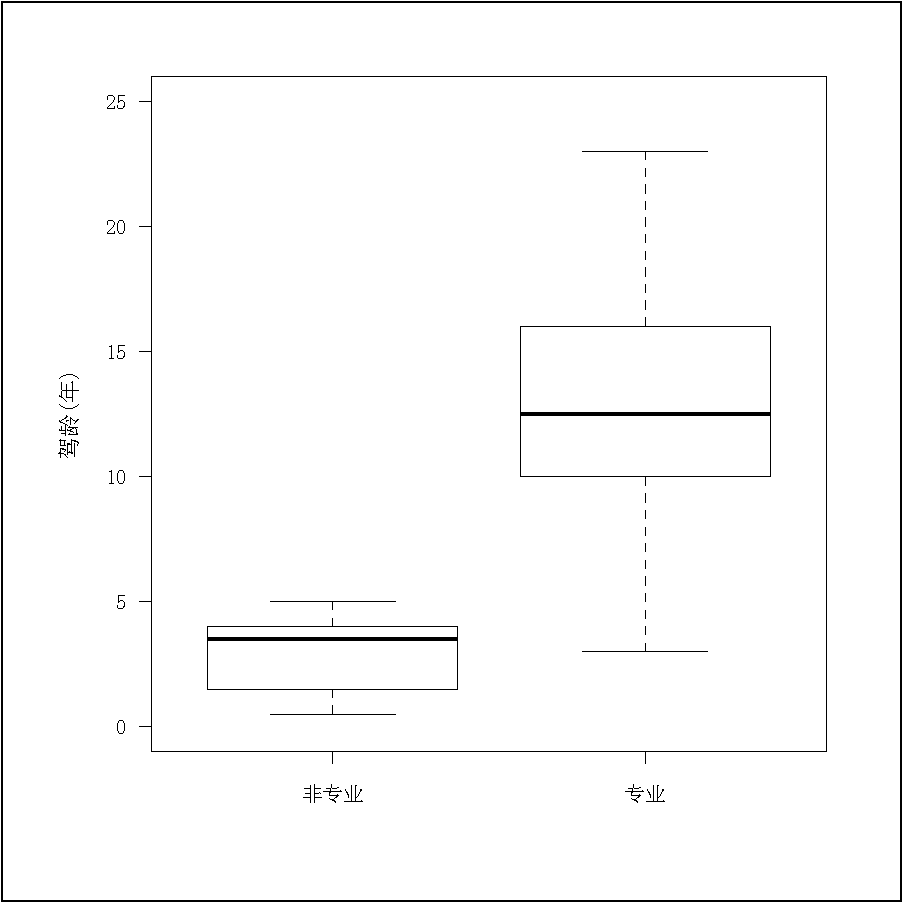
\includegraphics[width=\textwidth]{chapter4-certified_boxplot.pdf}
\caption{非专业与专业组驾龄箱图}
\label{certified_boxplot}
\end{minipage}%
\hspace*{0.04\linewidth}
\begin{minipage}[t]{0.48\linewidth}
\centering
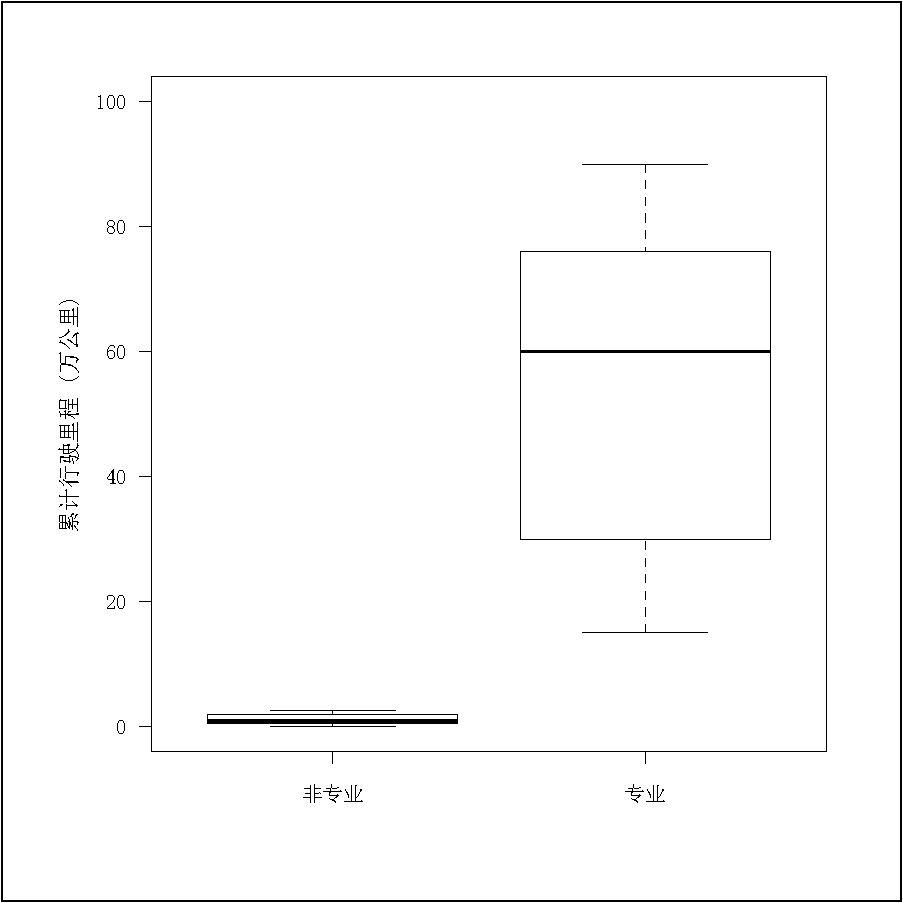
\includegraphics[width=\textwidth]{chapter4-mileage_boxplot.pdf}
\caption{非专业与专业组累计里程箱图}
\label{mileage_boxplot}
\end{minipage}
\end{figure}




\subsubsection{数据的基本情况}

通过实验获取共60041s(约16.6hr)的数据,就单个驾驶人而言最短的数据741s,最长的数据3623s。\autoref{d_density},\autoref{v_density}和\autoref{acc_density}分别给出了原始数据中测试车的跟驰距离,速度和加速度分布情况。由于城市路段交通情况的特点,跟驰距离主要集中在20米以内,峰值出现在2-6m之间。车速的分布,由于停车较多,速度为0的分布频次最多,而在0-40km/h的区间内分布比较平均,40-60km/h分布逐渐减少,很少有超过60km/h的车速。实验车加速度的分布峰值出现在0$m/s^2$,分布范围主要在[-2,2]$m/s^2$的区间。总体上数据的基本情况符合实际测试的交通状况。





\begin{figure}[htbp]
\begin{minipage}[t]{0.3\linewidth}
\centering
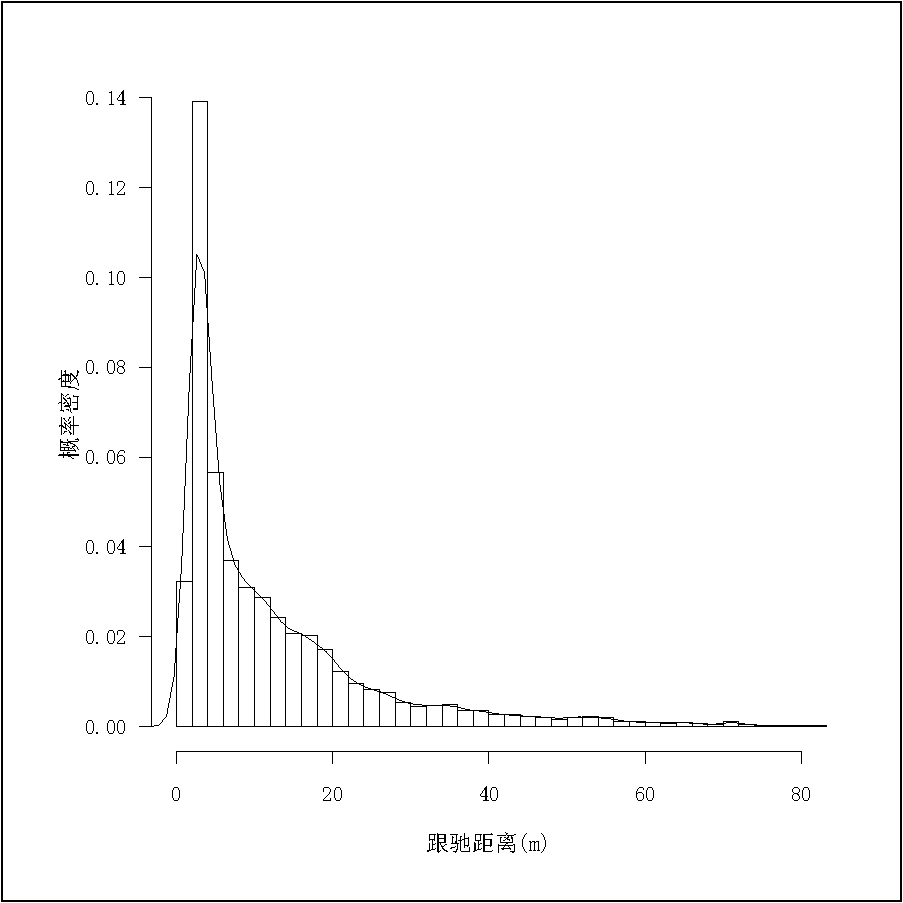
\includegraphics[width=\textwidth]{chapter4-d_density}
\caption{跟驰距离的核密度估计图}
\label{d_density}
\end{minipage}%
\hspace*{0.05\linewidth}
\begin{minipage}[t]{0.3\linewidth}
\centering
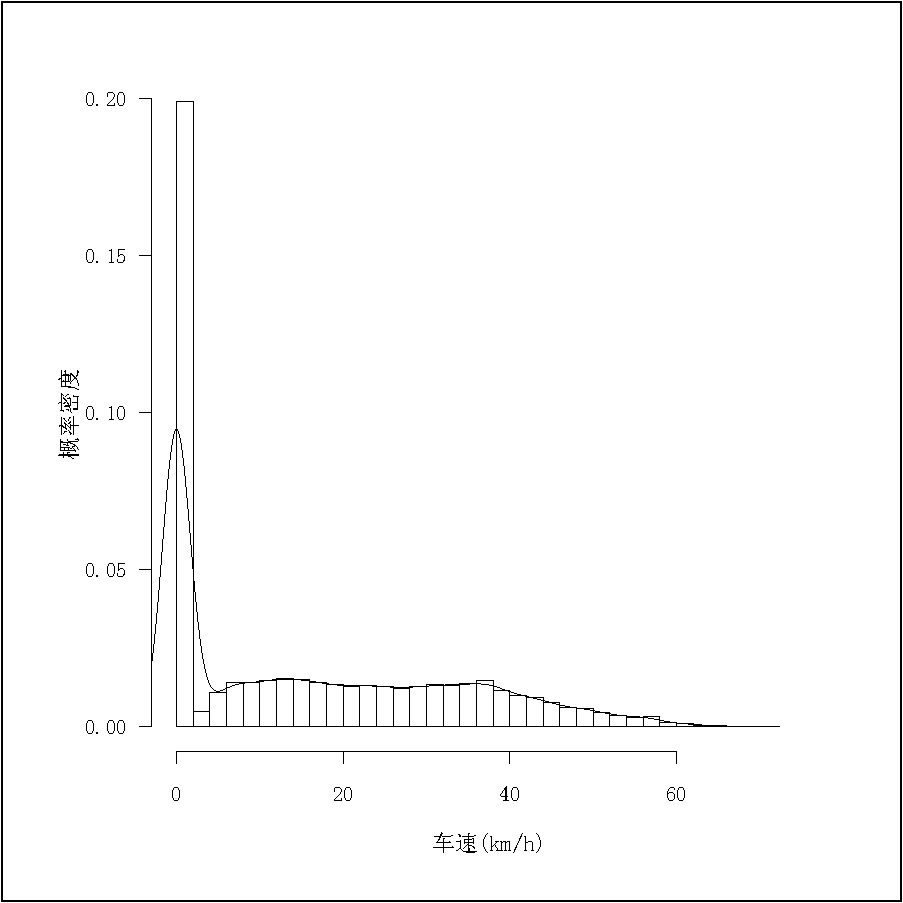
\includegraphics[width=\textwidth]{chapter4-v_density}
\caption{车速的核密度估计图}
\label{v_density}
\end{minipage}
\hspace*{0.05\linewidth}
\centering
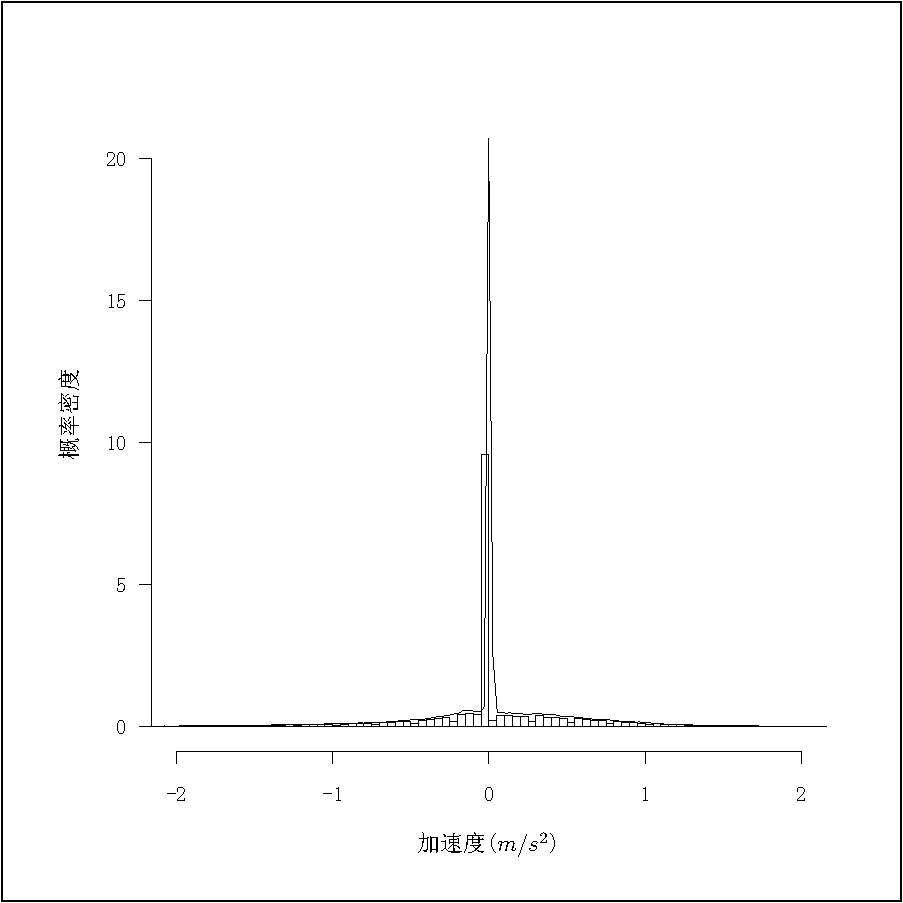
\includegraphics[width=0.3\linewidth]{chapter4-acc_density}
\caption{加速度的核密度估计图}
\label{acc_density}
\end{figure}







\subsection{数据处理}


由于激光测距系统的固有特性,所测的的原始数据中前车轨迹数据主要存在两方面的问题。其一,前车动态的数据不连续。激光测距测速仪安装于实验车上,在行驶过程中,受到前车尾部高度,反射率,车辆转向等因素的影响,其射出的光束并不能保证时刻得到有效的返回光束,因此也无法测出实验车与前车的相对动态关系。其二,所得数据存在随机误差(系统误差已通过试验设备的校准尽可能减小),随机误差理论上应符合正态分布,随机误差将使实验数据的分析发生偏差,Ossen(2008)\cite{Ossen2008}的实验表明,车辆轨迹的测量误差会对驾驶人行为参数的估计产生不可忽略的影响,因此有必要对数据进行后处理。对于车辆轨迹的后处理的最主要目的是得到对于真实轨迹的偏差尽可能小的估计。

目前研究中针对轨迹数据的处理主要有以下几种方法。

1.简单移动平均


最简单的轨迹数据后处理是简单移动平均,Thiemann等\cite{Thiemann2008}使用对称指数移动平均来平滑处理NGSIM的轨迹数据,发现了误差在差分过程中的放大效应,使得误差从位置,速度,加速度放大地向下传递,并使用移动平均来抵消这一效应。移动平均(低通滤波器)通常需要进行敏感性分析来确定移动平均的窗口大小和权重函数,从而使得既能够降低噪声又能保存原有信号中的高频部分。一般通过频谱分析来确定截断频率。

% The most basic filtering technique is the simple moving average. (16) use a 
% symmetric exponential moving average filter to smooth NGSIM data. They detect the magnification of noise 
% after differentiation and address it first by differentiating positions to speeds and accelerations and then by 
% smoothing all three variables. 
% Moving average generally needs a sensitivity analysis to find windows and weights that provide the 
% best tradeoff between the damping of the noise and the losing of high frequency parts of original trajectories. In 
% general, attention must be paid when using such techniques (or low-pass filters) since they may remove some 
% detailed information while leaving part of the noise. Therefore it would advisable if the choice and the design of 
% filters were preceded by spectral analysis of data. Such analysis can give useful information e.g. to decide the 
% most appropriate cut-off frequency and to design the frequency response of the filter. 

2.卡尔曼滤波

Ervin, R.等\cite{Ervin2000}使用卡尔曼滤波的方法对SAVME系统采集的轨迹数据进行了平滑处理,Punzo等\cite{Punzo2009}使用类似的方法对GPS采集的轨迹数据进行了处理。卡尔曼滤波需要对车辆的运行模型进行假设,而研究车辆的运行模型往往是采集轨迹数据的目的,因此若本文使用卡尔曼滤波进行轨迹数据的处理存在逻辑上的矛盾。
% The Kalman filter needs a simple traffic model and
% thus introduces some significant assumptions into the smoothing process. Also, the Kalman
% filter has more parameters while the sEMA method has only one parameter, T, and does not
% introduce complicated assumptions.

% Ervin et al. (6, 7) used Kalman
% filtering to smooth trajectory data collected by using video cameras
% with the SAVME system. Punzo et al. (8) used a similar approach
% with data collected by using GPS technology. The Kalman filter was
% applied with average speeds that were derived from the raw data.
% Thus, the result was smoothed average measurements rather than
% instantaneous ones. Although the difference between the two types
% of measurements may be negligible for the very short time intervals
% (0.1 s) reported in their application, it is expected to be more signif-
% icant for longer intervals. Furthermore, with the SAVME system, the
% Kalman filter is based on a model of the vehicle dynamics. However,
% the development of such model is, in most cases, the purpose of the
% data collection effort.

3.局部加权回归

Toledo等\cite{Toledo2007a}提出了使用局部加权回归的方法对轨迹数据进行处理的方法,局部加权回归可以较好地使用多项式拟合高度非线性的函数,可以用来处理轨迹数据和速度数据。Toledo等\cite{Toledo2007a}的研究表明局部加权回归结果对于参数选择,测量误差和缺失测量值均是较为稳定的。
% The approach uses local regression, a
% method well suited for mapping highly nonlinear functions. The proposed
% methodology is applied to a set of position data. The results demonstrate
% the value of the method to development of vehicle trajectories and speed
% and acceleration profiles. The conducted sensitivity analysis also shows
% that the method is rather robust regarding measurement errors and
% missing values.

本文中根据所测数据的特性,比较各种方法后选取局部加权回归的方法对轨迹数据进行处理,并根据一定的原则通过筛选,获取合理的数据。


%介绍local regression的原理和作用
\subsubsection{局部加权回归}
Cleveland\cite{Cleveland1979}最早提出了局部加权回归的方法,局部加权回归在每一点使用数据的一个子集(一般选取以拟合点中心对称的一个“窗口”)通过低阶的多项式函数进行拟合,多项式系数的估计采用加权最小二乘法,对于靠近拟合点的数据给予较高的权重而远离拟合点的数据则反之,得出拟合函数后计算拟合点的数值。局部加权回归可以灵活的选取窗口大小和权重函数以适应不同的应用需求。
% At each point in the data set a low-degree polynomial is fitted to a subset of the data, with explanatory variable values near the point whose response is being estimated. The polynomial is fitted using weighted least squares, giving more weight to points near the point whose response is being estimated and less weight to points further away. The value of the regression function for the point is then obtained by evaluating the local polynomial using the explanatory variable values for that data point. The LOESS fit is complete after regression function values have been computed for each of the n data points. Many of the details of this method, such as the degree of the polynomial model and the weights, are flexible. The range of choices for each part of the method and typical defaults are briefly discussed next.


对前车数据应用局部加权回归时,需要进行3个参数的选择,分别是权重函数,多项式次数和窗口大小。

根据实际情况,本文处理中权重函数选取了Tricube核函数,
\begin{equation}
w(t_0,t)=(1-u(t_0,t)^3)^3
\end{equation}

\begin{equation}
u(t_0,t)=\frac{\left | t-t_0 \right |}{d}
\end{equation}

其中:
\begin{displaymath}
{\begin{aligned}
w(t_0,t)&=\text{中点为}t_0\text{时}t\text{点的权重}\\
u(t_0,t)&=t\text{到}t_0\text{的规格化距离}\\
d&=t_0\text{到窗口外最近一点的距离}\\
\end{aligned}}
\end{displaymath}



其形状如\autoref{tricub}

\begin{figure}[htbp]
\begin{minipage}[t]{0.48\linewidth}
\centering
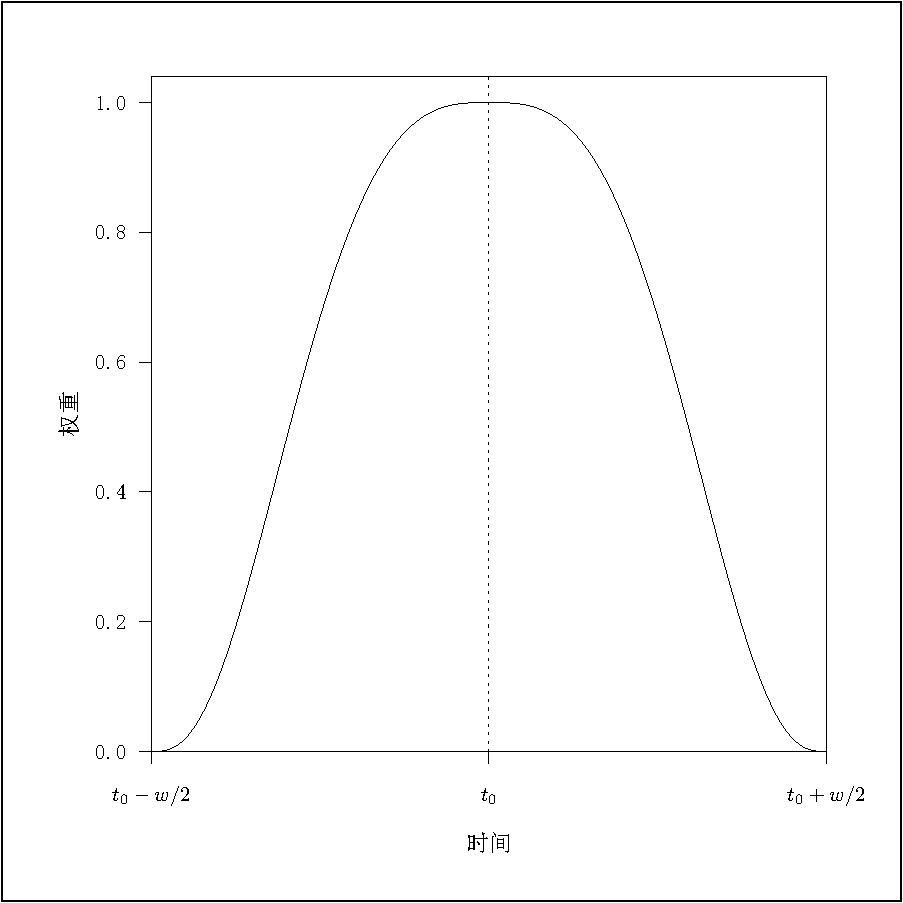
\includegraphics[width=\textwidth]{chapter4-tricub}
\caption{Tricube核函数示意图}
\label{tricub}
\end{minipage}%
\hspace*{0.04\linewidth}
\begin{minipage}[t]{0.48\linewidth}
\centering
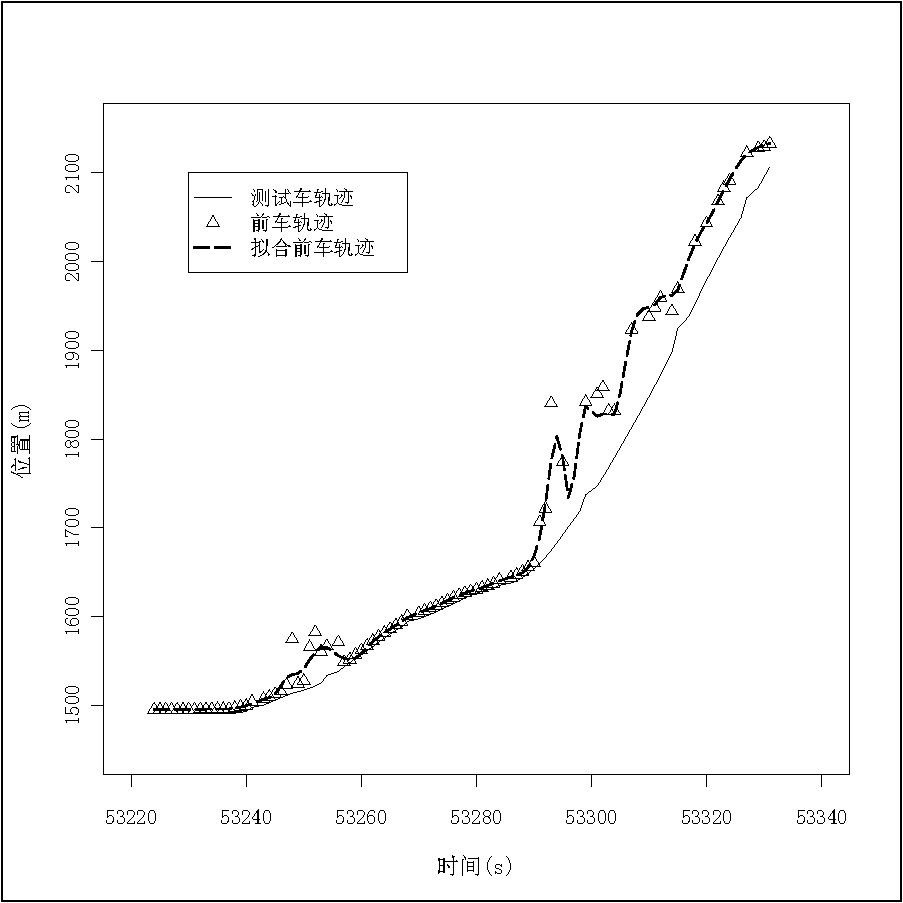
\includegraphics[width=\textwidth]{chapter4-sample-processing}
\caption{前车(引导车)轨迹数据局部回归示意图}
\label{sample-processing}
\end{minipage}
\end{figure}


为了保证回归后所得数据的合理性,需要保证回归多项式次数至少为3次,从而当从轨迹数据求导获取速度和加速度数据时,速度和加速度不会退化为常数。而过高的次数会增加计算的复杂度,并且高次多项式需要更大的数据窗口进行拟合,因此本文中选取多项式次数为3,窗口大小选择为11个数据点,一般会覆盖到1s的时间。


经过局部回归处理后的数据,还需要对数据进行筛选,合理的前车轨迹数据应符合以下两个条件,其一由于正常行驶中车辆不后退,因此轨迹数据应为非严格单调增函数;其二由于车辆运动的宏观连续性,拟合数据与原始数据较大的差值往往表明原始数据中前车运动已经超过可能的物理极限,为无效数据,因此有效的局部回归数据应与原始数据较为吻合。其三前车数据应符合交通情况和物理极限,例如车速超过60km/h和加速度在[-5,10]$m/s^2$之外的应为无效数据。


\autoref{sample-processing}为对前车轨迹数据处理的样例,例如图中53260s到53290s的数据为回归拟合较好的数据,而53300s周围的数据由于出现车辆倒退为无效数据,需要排除在有效数据之外。


\subsubsection{处理结果}
\label{process-result}
%start from here 2011
经过数据处理与数据筛选后,60041s的数据中共24374s大约40.6\%的数据成为最终用于分析的数据。经过处理后的数据中实验车数据的跟驰距离,车速和加速度分布如\autoref{postprocess-d-density},\autoref{postprocess-v-density}和\autoref{postprocess-acc-density}


\begin{figure}[htbp]
\begin{minipage}[t]{0.3\linewidth}
\centering
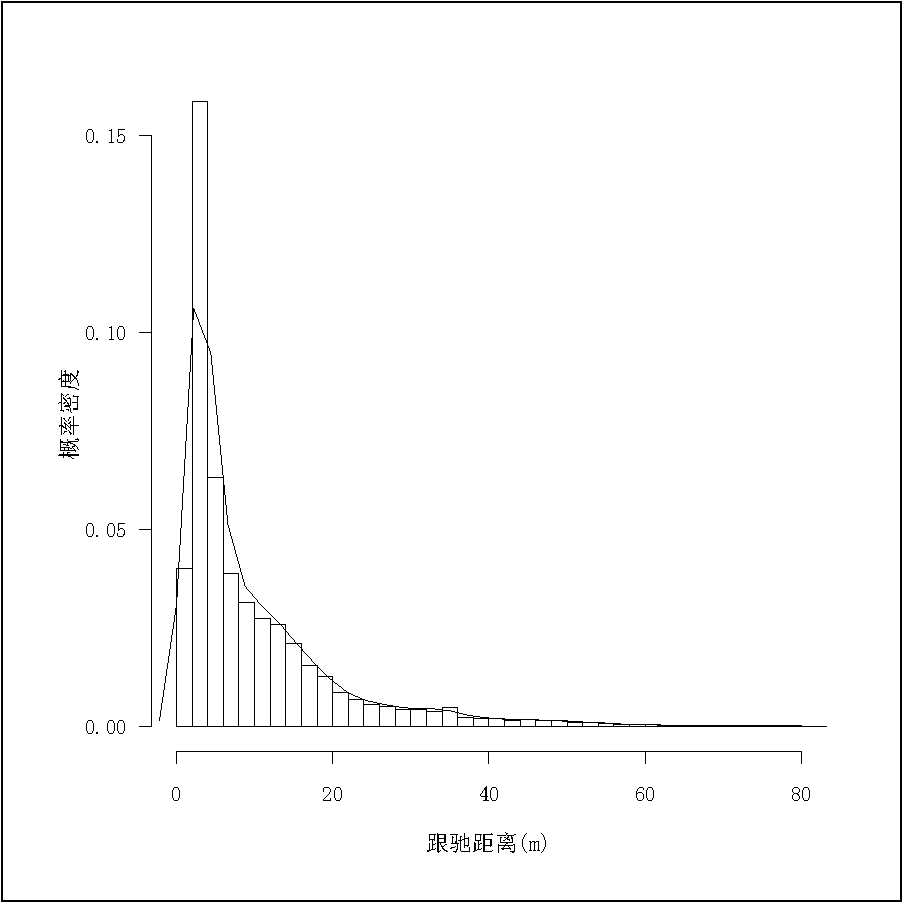
\includegraphics[width=\textwidth]{chapter4-postprocess-d-density}
\caption{处理后跟驰距离概率核密度估计图}
\label{postprocess-d-density}
\end{minipage}%
\hspace*{0.05\linewidth}
\begin{minipage}[t]{0.3\linewidth}
\centering
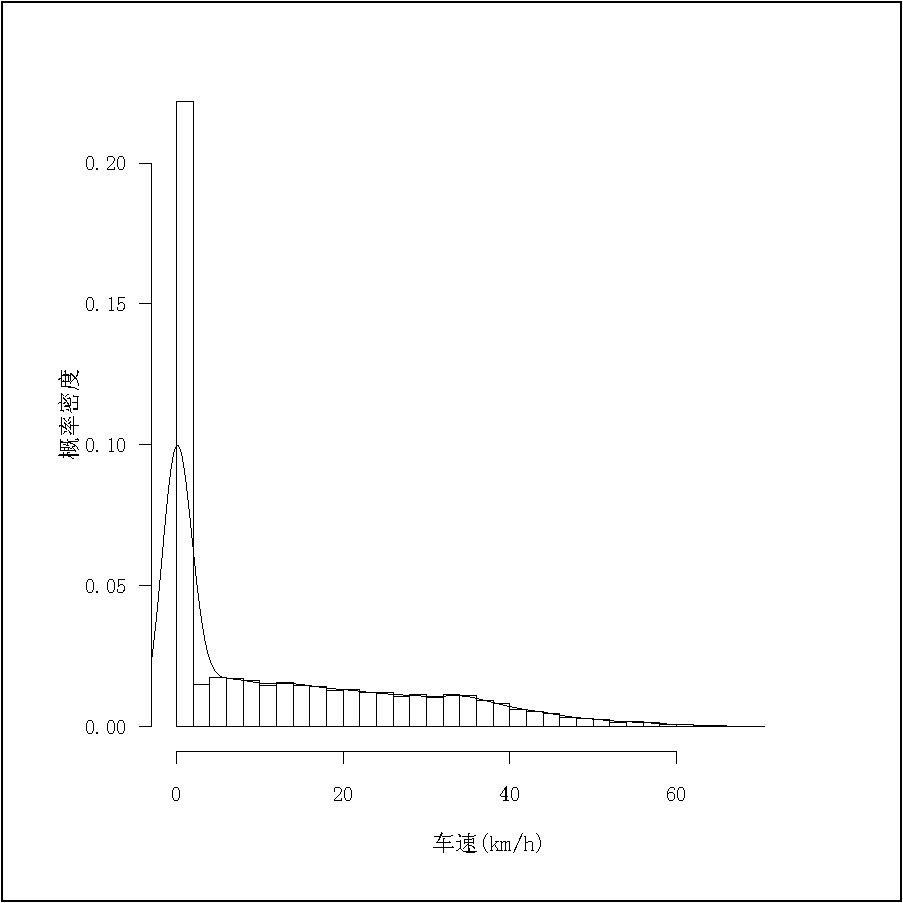
\includegraphics[width=\textwidth]{chapter4-postprocess-v-density}
\caption{处理后速度概率核密度估计图}
\label{postprocess-v-density}
\end{minipage}
\hspace*{0.05\linewidth}
\centering
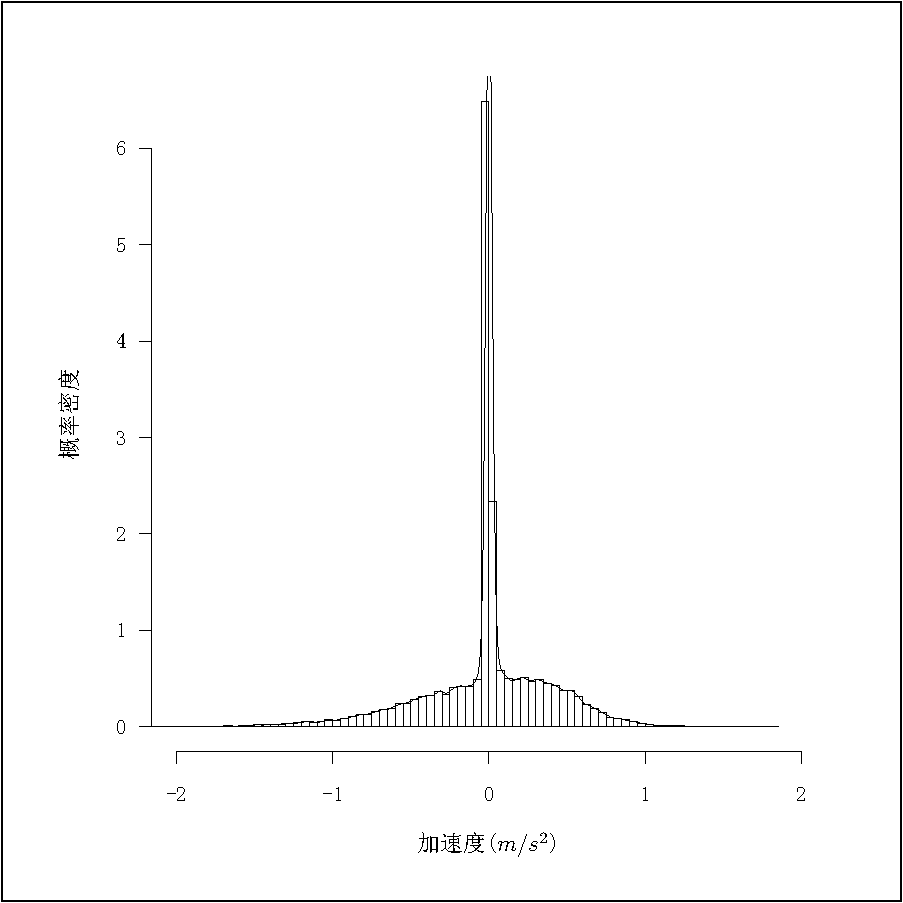
\includegraphics[width=0.3\linewidth]{chapter4-postprocess-acc-density}
\caption{处理后加速度概率核密度估计图}
\label{postprocess-acc-density}
\end{figure}


处理后的数据参数分布,其形状对比\autoref{d_density},\autoref{v_density},\autoref{acc_density},可以看出数据处理并未对数据的固有特征造成显著的影响,因此可以认为数据处理未对原始数据进行有偏差的抽取。

%\section{问卷信息}
\section{跟驰行为特性的集计分析}
本节通过对数据的集计,对专业与非专业驾驶人的行为特性进行初步的分析,从而研究专业与非专业驾驶人驾驶行为的异同。分析主要针对三个方面,一,自由流与跟驰的临界点;二,稳定状态下跟驰距离与速度的关系;三,加速度与车辆相互运动的关系。

\subsection{自由行驶与跟驰的临界点}
% Discerning free driving from car-following state plays an essential role in modeling driver’s car-following behavior. Many car following models distinguish free driving from car following state, and assume that a driver tends to drive at a desired speed until getting influenced by vehicles ahead of him. It is also conceivable that the influence of frontal vehicle is larger for short time/space distance and smaller for longer time/space distance. But how distant away a driver starts to engage frontal vehicle and get into car-following state has not been fully studied. 

车辆的行驶可认为存在自由行使和跟驰两种状态,自由行驶是指车辆在不受前车影响下的自由行驶。而跟驰情况下,车辆速度受到前车速度的影响。一般可以假设认为,前车对于驾驶人的影响大小与其时间或空间意义上的距离有关,距离越小则影响越大而距离越大则影响越小。自由行驶和跟驰的临界点是影响跟驰行为的重要因素,因此也是反映驾驶人行为特性的一个指标。

% Based on the obtained data the method proposed by K. Vogel was used to determine the threshold between free driving and car following. The reasoning of the scheme is briefly described as follows.
% The criterion for separating ‘‘free’’ and following vehicles is that the speed of a free vehicle should not be influenced by the speed of the vehicle ahead. Thus, the speeds of the two vehicles should not correlate.
Vogel(2002)\cite{Vogel2002}提出了通过定点测量的车头时距和车速数据确定自由行驶与跟驰的临界点的方法,根据车头时距和车头间距对数据进行分组,其后计算每组数据内前后车速度的相关系数来代表前车对后车速度的影响程度。其数据表明当车头时距大于一定数值后,车速的相关系数出现突然的下降,通过假设临界点分别对假设的跟驰数据和自由行使数据进行线性拟合试算,当两组数据的拟合的交点与分割点最为接近时则认为得到了自由行驶与跟驰的临界点。

本文中针对所获取的数据,基于Vogel的方法,使用时间间隔替换车头时距分别对专业和非专业驾驶人的数据进行了自由行驶与跟驰的临界点的确定。
对于所有的数据,将时间间隔数据舍入到最近的秒数,例如时间间隔在0.5至1.5秒坐开右闭区间的归入到1秒的组别,在1.5至2.5秒坐开右闭区间的归入到2秒的组别,依此类推。对于超过20.5秒的数据由于数据量很少不能得到可靠的速度相关系数值,因此排除在考察数据之外。

对专业和非专业驾驶人,分别计算速度相关系数,并进行线性回归的试算,其结果如\autoref{tab-free-discern},回归示意图如\autoref{nonpro-tgap-discern}和\autoref{pro-tgap-discern}。

\begin{table}[htbp]
  \centering
  \caption{自由行驶与跟驰临界点结果表}
    \begin{tabular}{ccc}
    \addlinespace
    \toprule
          & 专业驾驶人 & 非专业驾驶人 \\
    \midrule
    临界点时间间隔 & 6.5s  & 11.5s \\
    跟驰拟合R平方 & 0.9899 & 0.9925 \\
    自由行驶拟合R平方 & 0.3302 & 0.0892 \\
    交点 & 6.06s & 11.34s \\
    跟驰拟合方程 & y=-0.06526x+ 0.93158 & y=-0.0679x+ 0.9996 \\
    自由行驶拟合方程 & y=-0.02613x+ 0.69439 & y=-0.00752x+ 0.31514 \\
    \bottomrule
    \end{tabular}%
  % \label{tgap-discern}%
\label{tab-free-discern}
\end{table}%

\begin{figure}[htbp]
\begin{minipage}[t]{0.48\linewidth}
\centering
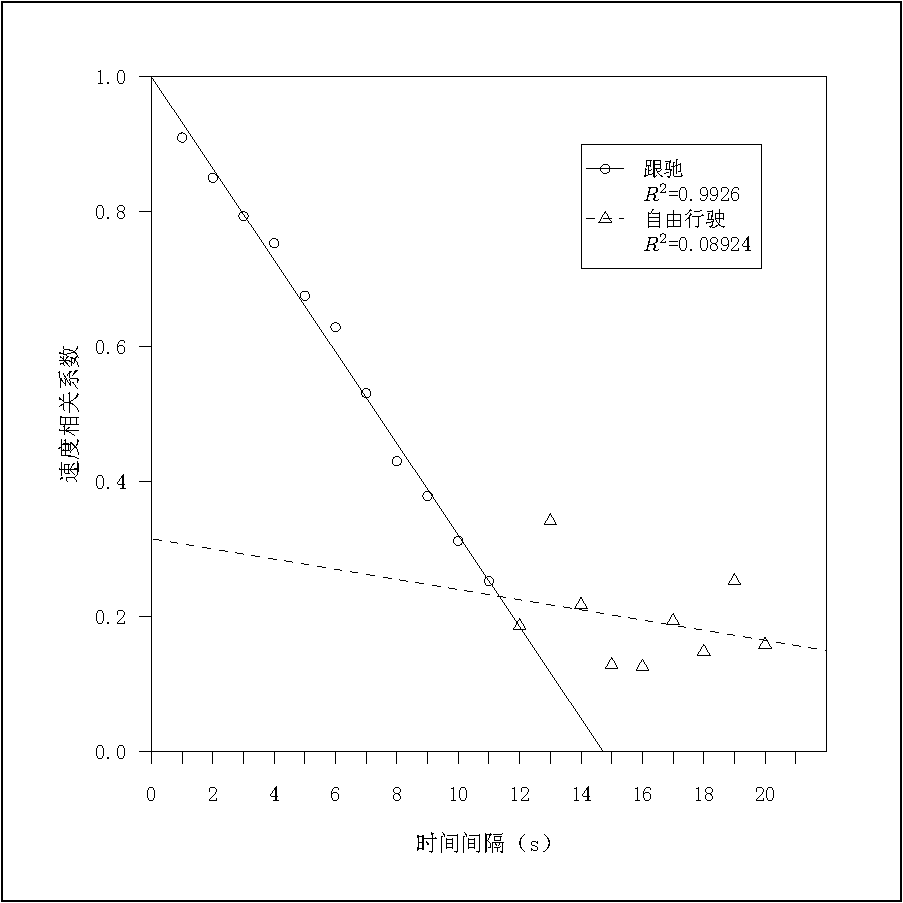
\includegraphics[width=\textwidth]{chapter4-nonpro-tgap-discern}
\caption{非专业驾驶人时间间隔-速度相关系数图}
\label{nonpro-tgap-discern}
\end{minipage}%
\hspace*{0.04\linewidth}
\begin{minipage}[t]{0.48\linewidth}
\centering
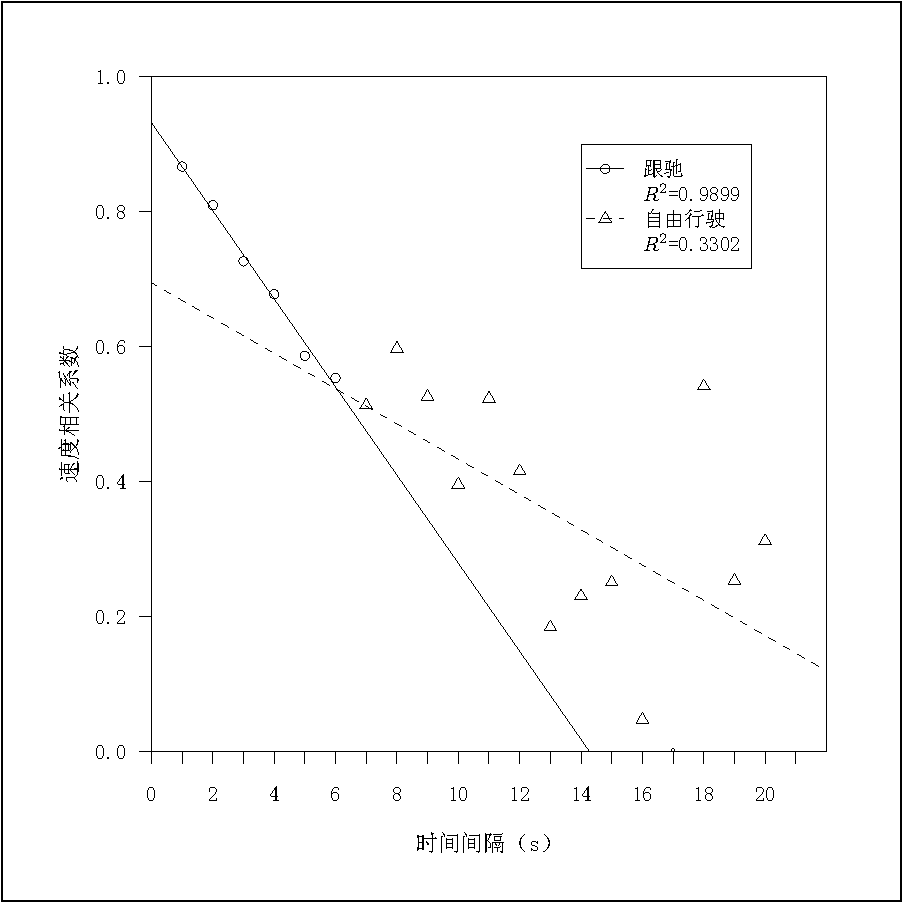
\includegraphics[width=\textwidth]{chapter4-pro-tgap-discern}
\caption{专业驾驶人时间间隔-速度相关系数图}
\label{pro-tgap-discern}
\end{minipage}
\end{figure}





% Upon this approach, the criterion for determining the cut-off point for free and following vehicles would be the x-axis value of the intercept point of the two regression lines. It should be as close as possible to the time/space distance value which was used to split the data into the two subgroups. If this were not the case, it would indicate that the division was not made at the correct location. The empirical data would need to yield a drop in correlation values at the threshold. Therefore it is basically the task to find regression lines that intersect close to the split point to get the threshold.

% For all observations the time gap was rounded to the nearest second, and then grouped according to time gap. For example, vehicles with time gaps between 0.5 s (excluded) and 1.5 s (included) fell into group 1 with a rounded time gap of 1 s, vehicles with a time gap between 1.5 (excluded) and 2.5 s (included) fell into group 2 with a rounded time gap of 2 s, and so on. Vehicles with time gaps that are longer than 20.5 s were too scarce to provide reliable estimate of speed correlation and are excluded. 

% For the two drivers’ groups, in each time gap interval the speed correlation was calculated. The correlation values of the two drivers’ group are plotted in Fig and Fig; for each driver’s group the speed correlations all decreased while time gaps increased. However, they show quite different patterns. 
% For the experienced group with a time gap of 1 s the correlation value was about r=0.9, i.e. more than 80% of the variance in speed was explained by the speed of the vehicle ahead. For each additional second in time gap, up to 6 s, the correlation value r decreased substantially. For time gaps of more than 6 s and less than 12 s the correlation values started to fluctuate but still decreased in trend, and the slope was not as steep as before 6 s. For time gaps of more than 12 s the speed correlation went under 0.4.

% For beginners group with a time gap of 1s the correlation value was also about r=0.9. For each additional second in time gap, up to 12s, the correlation value r decreased substantially, for time gaps of more than 12s the curves appear to level out. For headways of 12s and longer, the speed of frontal vehicle accounted for no more than 10% of the speed of subject vehicle.
结果显示,对于专业驾驶人1s的时间间隔其速度相关系数为0.9,也就是说超过80\%的泵车速度变化可以由前车的速度解释,到6s之前每增加1s的时间间隔,速度相关系数均显著下降。在6s与12s之间速度相关系数产生一些波动,总体上仍呈现下降趋势。超过12s后速度相关系数减小到0.4以下;对于非专业驾驶人,1s的时间间隔其速度相关系数也约为0.9,直到12s速度相关系数均显著下降,超过12s后速度相关系数减小到0.1以下。
% Based on these observations, for each driver group possible split points were chosen. One linear regression was computed on the correlation values below the split point; another linear regression was computed above the split point. The best split point turned out to be 6.5 s and 11.5 s for experienced and beginner group respectively. Results are provided in Table 1, regressions are shown in Figure. 5 and Figure. 6 
从专业与非专业自由行驶与跟驰临界点结果看,专业驾驶人的临界点为6.5s,非专业驾驶人为11.5s,这似乎意味着非专业更早的受到前车的影响而进入跟驰的状态,但是结合速度相关系数的数值,在(6.5,11.5]的时间间隔区间内,专业驾驶人的速度相关系数要大于非专业驾驶人的相应数值。将(6.5,11.5]的时间间隔区间内的数据选出,得到专业驾驶人8159组数据,非专业驾驶人7245组数据,计算前后车辆的速度差值,两组数据基本上呈正态分布。分别统计得到专业驾驶人速度差中位数为0.3281m/s,标准差4.357m/s;非专业驾驶人速度差中位数为0.3677m/s,标准差4.801m/s。通过Levene检验,专业组与非专业组的速度差方差存在统计意义的显著差别(P<0.01)。以上结果表明在(6.5,11.5]的时间间隔区间内,驾驶人仍然有与前车保持速度一致的趋势,同时专业驾驶人的速度差分散程度要小于非专业驾驶人。综合所得结果可以推断,对于专业和非专业驾驶人在一定的时间间隔内,均受到前车速度影响,相比于非专业驾驶人专业驾驶人似乎能更好地将自身的车速与前车保持一致,尤其是在稍大的时间间隔区间。
%,因此可以认为专业驾驶人有更为“平滑”的驾驶特性。
%The results presented above suggest a 6.5s time gap separation between free driving and car following for the experienced group and accordingly 11.5s for the beginners group. It would seem that beginner drivers start to engage leading vehicle earlier in the time gap sense than experienced drivers. However, the results needs careful interpretation. Although the separation point for the experienced group is 5s longer than that of the beginners group, the speed correlation for the experienced group was generally larger in between the (6.5,11.5] time gap section. For both group the speed correlation dropped almost linearly as time gap increase before the separation point. Before the separation point, time gap all explained over 90% variance of speed correlation. But above the separation point, time gap only accounted for less than 10% of the speed correlation variance for beginners group, yet accounted for 33% of the speed correlation variance for experienced group. Based on the findings,  it is possible to surmise drivers do not differ in perceiving influence from frontal vehicle but differ in taking action. Thus it would be reasonable to choose 12s time gap to be a separation point between free driving and car-following.
% The 12s time gap value is greater than the former proposed 6s time headway value reported by K. Vogel. This clearly suggests the separation point between free driving and car-following is not universal. The variation could come from different sources, e.g. the different road and traffic conditions, different driving behaviors and certainly the different technology used to measure the behavioral data. In order to account for this variation , further investigation is needed and should focus on the influence of different road and traffic conditions.
%In addition, the patterns showed in Figs indicate a difference between the two driver groups. Further analysis was done to explore the difference between driver groups. Data in the (6.5, 11.5] time gap section was picked out for both groups. The experienced group consisted of 8159 observations and the beginners group consisted of 7245 observations. The speed difference (speed of leading vehicle minus speed of subject vehicle) of each observation was calculated for both groups. Central tendency of speed differences was given by the median value: 0.3677m/s for beginners and 0.3281m/s for experienced drivers and sample standard deviations were 4.801 and 4.357 respectively. The low median values suggest drivers tend to adapt their speed to frontal vehicle in the (6.5, 11.5] time gap section. Levene’s test was performed to check the equality of variances. The result showed the speed difference variance of the two groups differed significantly (P<0.01). This combined with the S.D. values indicate experienced drivers adapt his speed to frontal vehicle better.


\subsection{稳定状态下跟驰距离与速度的关系}
%speed-distance profile
速度-跟驰距离选择反应了驾驶人跟驰行为特性中相对稳定的部分,驾驶人根据出行计划,道路条件,交通流条件来选择车速,当车辆的加速度小于一定的阈值时则认为处于稳定的跟驰状态,此时驾驶人根据其选择的车速会与引导车保持一定的跟驰距离。

基于稳定状态下跟驰距离与速度有关的假设,将实验中所获取的数据加速度绝对值小于0.1$m/s^2$的数据选出并分组集计:分别对专业组和非专业组驾驶人按照速度分组,计算每组相应的平均跟驰距离和平均速度,其关系如\autoref{stable-v-distance}。

由\autoref{stable-v-distance}可以看出,整体上跟驰距离随车速的增加而增加,这符合一般认识。对平均车速和平均跟驰距离进行线性回归,得到回归方程。对于专业驾驶人$d_1(m)=1.557 v_1(m/s) + 3.8652$,其$R^2=0.3277$。对于非专业驾驶人$d_2(m)=1.830 v_2(m/s) + 2.6901$,其$R^2=0.4466$

\begin{figure}[htbp]
\begin{center}
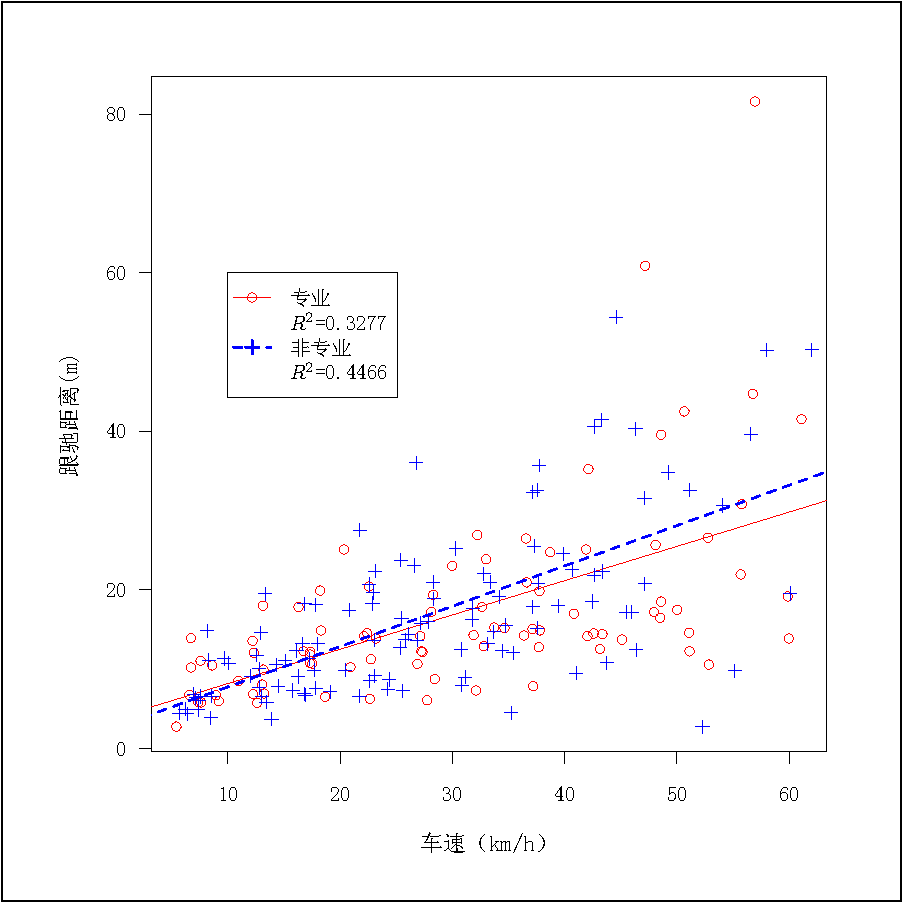
\includegraphics[width=0.6\linewidth]{chapter4-stable-v-distance}
\end{center}
\caption{稳定状态下跟驰距离与速度关系图}
\label{stable-v-distance}
\end{figure}

通过设置虚变量可以检验(T检验)专业组和非专业组的回归系数的差异是否显著。设置虚变量$PRO$,对专业驾驶人$PRO=1$,非专业驾驶人$PRO=0$,则通过回归:
\begin{equation}
d=h_1 \cdot PRO+h_2\cdot v + h_3 \cdot PRO \cdot v +b
\end{equation}
其中$h_1$为截距差,$h_3$为斜率差。

得到\autoref{h-b-df},结果表明两组线性回归的斜率与截距均无统计意义的显著差异(P=0.05)水平下,不能拒绝$h_1=0$或$h_3=0$的假设)。因此此处集计分析的证据,不能支持专业与非专业驾驶人的稳定状态下跟驰距离与速度关系特性存在显著差异的观点。

\begin{table}[htbp]
\begin{center}
\caption{专业组和非专业组的跟驰距离与速度关系回归系数的差异显著性检验}
\begin{tabular}{rrrrr}
  \addlinespace
  \toprule
 & 估计值 & 标准误差 & t值 & P值 \\ 
  \midrule
b & 2.69 & 1.83 & 1.47 & 0.14 \\ 
  $h_1$ & 1.18 & 2.77 & 0.42 & 0.67 \\ 
  $h_2$ & 1.83 & 0.21 & 8.75 & 0.00 \\ 
  $h_3$ & -0.27 & 0.30 & -0.90 & 0.37 \\ 
   \bottomrule
\end{tabular}
\label{h-b-df}
\end{center}
\end{table}


\subsection{加速度与车辆相互运动的关系}
\label{ttc}
%acceleration-speed-difference profile
加速度与车辆相互运动的关系反应了驾驶人跟驰行为特性中相对不稳定的部分。按照刺激反应模型的假设,驾驶人在一定的相对速度下选择相应的合适的加速度,当与前车有接近趋势时则选择负的加速度,有远离趋势时选择正的加速度,而驾驶人采取的加速度与受到的刺激(速度差)成正比。一般化的GM模型认为加速度不仅与速度差有关还与跟驰距离以及车速有关。


Xin等(2008)\cite{Xin2008}提出了驾驶人加速度模型,认为驾驶人的与前车的视觉扩张率有关,但是未明确指出其关系。其视觉扩张率指,物体投射在视网膜上的角度的变化率,
\begin{equation}
tan(\frac{\theta}{2})=\frac{W/2}{D(t)}
\end{equation}

\begin{equation}
\frac{sin(\theta)}{\dot{\theta}}=\frac{D(t)}{\Delta V}
\end{equation}
其中:



\begin{displaymath}
{\begin{aligned}
\theta&=\text{前车投射在视网膜上的角度}\\
\dot{\theta}&=\text{前车投射在视网膜上的角度的变化率即视觉扩张率}\\
W&=\text{前车宽度}\\
D(t)&=t\text{时刻的车头间距}\\
\Delta V&=\text{相对速度}\\
\end{aligned}}
\end{displaymath}


在驾驶过程中前车投射在驾驶人视网膜上的角度较小,因此视觉扩张率可以近似为:
\begin{equation}
\theta \approx \frac{W}{D}
\end{equation}


\begin{equation}
\frac{\theta}{\dot{\theta}}=\frac{D(t)}{\Delta V}
\end{equation}

\begin{equation}
\dot{\theta}=W\frac{\Delta V}{D^2}
\end{equation}

在交通冲突技术中Time-To-Collision(TTC)被证明是有效的度量交通冲突严重程度的手段。Hayward(1972)\cite{Hayward1972}定义TTC为;“两车保持当前速度和路线而相撞所需要的时间。”Lee(1976)\cite{Lee1976}定义TTC为两物体距离比上其相对速度。Balas和Balas(2006)\cite{Balas2006}比较了TTC倒数和TTC,认为TTC倒数比TTC更为直接和连续的反映了碰撞的危险,并且认为TTC倒数可用于解释驾驶人的驾驶行为。

基于加速度与速度差跟驰距离有关的观点,假设前车宽度基本不变,将实验中所获取的数据分组集计:分别对专业组和非专业组驾驶人按照速度差距离比$\frac{\Delta V}{D}$即TTC倒数,加速度与速度差距离平方比$\frac{\Delta V}{D^2}$进行分组,计算每组相应的平均速度差距离比,平均速度差距离平方比,以及平均加速度,得到关系如\autoref{a-deltavbyd}和\autoref{a-deltavbyd2}。

\begin{figure}[htbp]
\begin{minipage}[t]{0.48\linewidth}
\centering
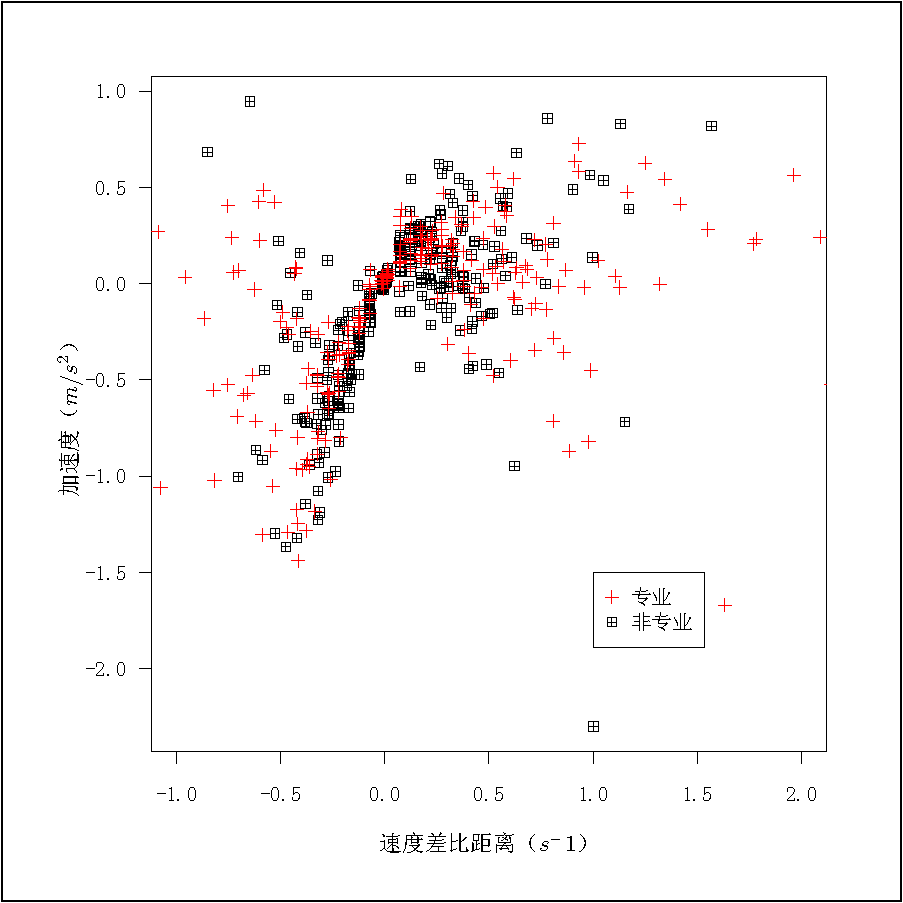
\includegraphics[width=\textwidth]{chapter4-a-deltavbyd}
\caption{加速度与速度差距离比图}
\label{a-deltavbyd}
\end{minipage}%
\hspace*{0.04\linewidth}
\begin{minipage}[t]{0.48\linewidth}
\centering
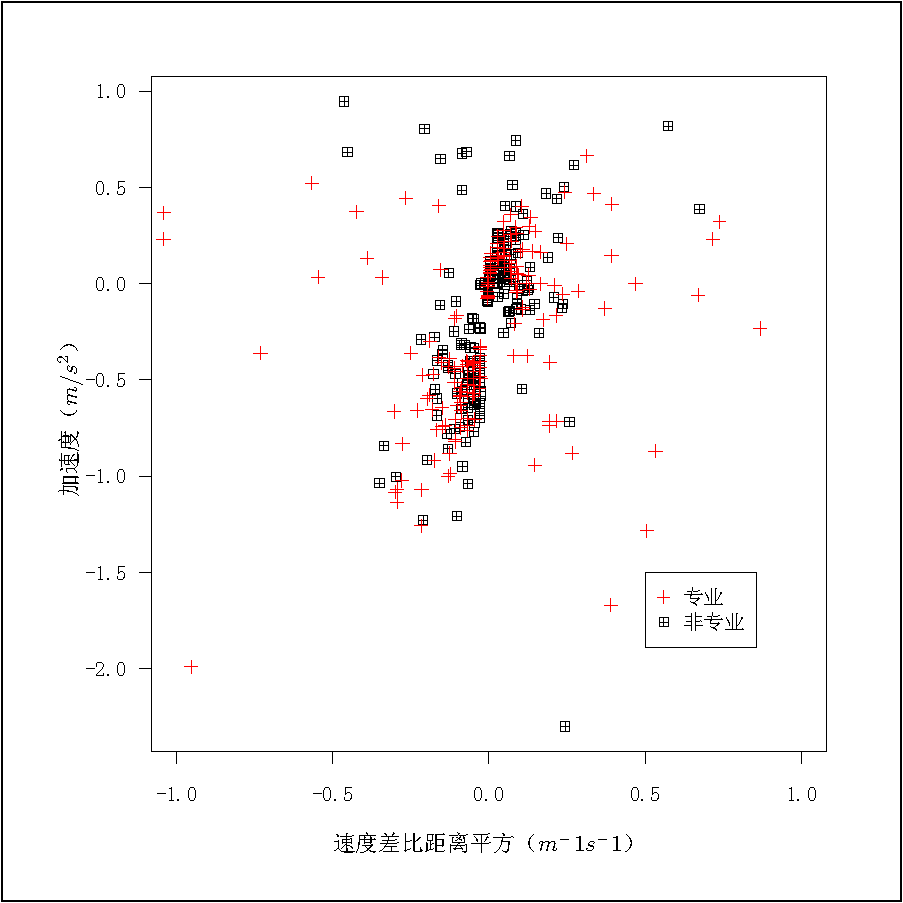
\includegraphics[width=\textwidth]{chapter4-a-deltavbyd2}
\caption{加速度与速度差距离平方比图}
\label{a-deltavbyd2}
\end{minipage}
\end{figure}


对于前车速度小于跟驰车辆的情况,由\autoref{a-deltavbyd}和\autoref{a-deltavbyd2}中的速度差轴左侧可以发现速度差距离比(TTC倒数)与驾驶人的负减速度存在明显的线性关系,说明驾驶人对于减速情况减速度的选择与速度差距离比有较大的相关性。而加速度与速度差距离平方比的线性关系则较不明显。而当速度差为正时驾驶人的加速度的分布均十分的分散,这表明驾驶人减速与加速之间存在不对称性。同时专业组和非专业组之间并未表现出明显的差别。


\subsection{集计分析小结}
从集计分析的结果可以发现专业和非专业驾驶人驾驶行为特性的差异得到了混合的结果,在自由行驶与跟驰的临界点方面存在明显的差别,而在稳定状态下速度与跟驰距离,加速度与车辆相互运动的关系特性方面不存在明显的差别。

%一方面可能是样本的代表性问题,专业组和非专业组的差别除了驾驶经验以外还有年龄和职业等的差异,因此专业组与非专业组的区别并不是一个单纯的影响因子。

由于集计分析忽略了更多驾驶条件的影响,例如在相同的速度差条件下速度值不同采取的加速度可能也不同。由于集计对驾驶人不同驾驶条件下的数据进行了平均,因此还需要对数据进行进一步的分析。下一节中将从更加微观的角度分析,使用跟驰模型参数标定的方法,分析跟驰模型参数在驾驶人中的分布情况,并作出相应的分析和推断。



%因此不能排除驾驶人在组内的差异性,

%同时结果表明驾驶人自身在加速与减速过程存在显著的差异性。






\section{跟驰模型参数标定}
为了进一步研究驾驶人行为特性的异同,并且为通过模拟研究驾驶人行为特性对交通流影响提供依据,本节使用轨迹数据对微观跟驰模型参数进行标定,并使用Bootstrap方法对所得结果进行分析和推断。
\subsection{标定方法框架}
Ossen(2008)\cite{Ossen2008}给出了一般化的通过轨迹数据标定跟驰模型的框架:

以$z_n(t)$表示驾驶人n车辆的真实行驶状态,此状态一般包含车辆的位置$x_n(t)$与速度$v_n(t)$,以$\xi_n(t)$表示驾驶人n所面临的交通条件,向量$\xi_n(t)$包含驾驶人n对于前方若干辆车的位置、速度等变量的观察和估计:

\begin{equation}
\xi_n(t)=(z_{n-j}(t),\cdots z_{n-1}(t))
\end{equation}

j为驾驶人n向前观测的车辆个数,本文数据由于技术原因只能测到向前一辆车的动态,标定中也将使用单引导车模型,因此:
\begin{equation}
\xi_n(t)=z_{n-1}(t)
\end{equation}

驾驶人车辆纵向的运动可以用跟驰模型来描述则:
\begin{equation}
\frac{d}{dt}z_n(t)=f(\xi_n(t-T_r\mid\beta_n))
\end{equation}

则系统的变化方程为:
\begin{equation}
\hat{z}_n(t_k)=\left\{\begin{matrix}
y_n(t_1))& k=1\\
\hat{z}_n(t_{k-1})+\int_{t_{k-1}}^{t_k} f(\xi_n(s-T_r)\mid\hat{\beta}_n)ds& \text{其他}
\end{matrix}\right.
\end{equation}

标定的目标就是找到最优的参数$\beta^*_n$使得目标函数最小:
\begin{equation}
\beta^*_n=argmin_{\hat{\beta}_n}g(y_n,\hat{z_n})
\end{equation}

其中g为目标函数,数量化度量模型预测结果和真实结果的差别。

\subsection{跟驰模型}

跟驰模型选用IDM(Intelligent Driver Model)智能驾驶模型,IDM模型自提出以后由于其优良的特性被广泛研究,IDM模型参数较少且具有明确易理解的物理意义。IDM模型统一描述了自由行驶和跟驰,并且可以体现加速和减速的不对称性。



Treiber等(2000)\cite{Treiber2000}和Treiber和Helbing(2003)\cite{Treiber2003}假设加速度受到期望速度和期望跟驰距离的影响提出了IDM模型,其形式如下:
% assume that the acceleration is
%affected by both the desired speed and the desired minimum space headway. The
%model also incorporates the impact of vehicle capabilities, but ignores reaction
%time: 
\begin{equation}
a_n(t)=a_{max}\left[1-\left(\frac{V_n(t)}{DV_n(t)}\right)^4-\left(\frac{D_n(t)}{\Delta X_n(t)}\right )^2\right],
\end{equation}
其中$a_{max}$为车辆的最大舒适加速度。$V_n$为实际车速,$DV$为期望速度,$D_n$为期望跟驰距离,$\Delta X_n$为实际跟驰距离。

%其期望车头间距给出如下:
%
%\begin{equation}
%D_n(t)=\Delta X_n^*+V_n(t)T_n(t)+\frac{V_n(t)\Delta V_n(t)}{2\sqrt{a_{max}b_{max}}},
%\end{equation}

驾驶人车辆的加速度由两个部分组成,其趋向自由行驶部分的加速度为:
\begin{equation}
a_{max}\left[1-\left(\frac{V_n(t)}{DV_n(t)}\right)^4\right],
\end{equation}

受前车影响部分的加速度为:
\begin{equation}
-a_{max}\left[\left(\frac{D_n(t)}{\Delta X_n(t)}\right )^2\right],
\end{equation}
当实际的跟驰距离小于期望跟驰距离时,此项成为加速度的主要部分。

其期望车头间距给出如下:
\begin{equation}
D_n(t)=\Delta X_n^*+V_n(t)T_n(t)+\frac{V_n(t)\Delta V_n(t)}{2\sqrt{a_{max}b_{max}}},
\end{equation}
其中$\Delta X_n^*$为停车间距,$T_n$为期望车头时距,当距离较小时$\Delta X_n^*$占期望跟驰距离的主要部分,$T_n$期望车头时距体现了驾驶人对安全跟驰距离的一种期望。$b_{max}$为最大舒适减速度。在大多数情况下将减速度的绝对值限制在其以下。






\subsection{目标函数}

g为目标函数,数量化度量模型预测结果和真实结果的差别。本文中使用Theil's U作为目标函数,
\begin{equation}
g(y_n,\hat{z}_n)=\frac{\sqrt{\frac{1}{K} \sum\limits_{k=1}^{K}(y_n(t_k)-\hat{z}_n(t_k))^2}}{\sqrt{\frac{1}{K} \sum\limits_{k=1}^{K}(y_n(t_k))^2}+\sqrt{\frac{1}{K} \sum\limits_{k=1}^{K}(\hat{z}_n(t_k))^2}}
\end{equation}
其中$y_n$为实际观测值,$\hat{z}_n$为模型预测值,考虑到本文数据采集所使用的方法以及交通流状况,使用跟驰距离而不考虑将速度代入到$y_n$和$\hat{z}_n$中计算,理由是实验数据中直接测量的变量包括跟驰距离,而前车速度经过计算得出,误差经由一次求导会被放大。城市交通流状况存在较多的停车,以速度代入也将使目标函数对参数过于敏感不利于得到合理的标定值。

\subsection{优化算法与搜索范围}
本文使用遗传算法(genetic algorithm)对目标函数进行优化,遗传算法是计算数学中用于解决最优化的搜索算法,是进化算法的一种。进化算法最初是借鉴了进化生物学中的一些现象而发展起来的,这些现象包括遗传、突变、自然选择以及杂交等。

遗传算法通常实现方式为一种计算机模拟。对于一个最优化问题,一定数量的候选解(称为个体)的抽象表示(称为染色体)的种群向更好的解进化。一般解用二进制表示(即0和1的串)。进化从完全随机个体的种群开始,初代种群产生之后,按照适者生存和优胜劣汰的原理,逐代(generation)演化产生出越来越好的近似解,在每一代,根据问题域中个体的适应度(fitness)大小选择(selection)个体,并借助于自然遗传学的遗传算子(genetic operators)进行组合交叉(crossover)和变异(mutation),产生出代表新的解集的种群。这个过程将导致种群像自然进化一样的后生代种群比前代更加适应于环境,末代种群中的最优个体经过解码(decoding),可以作为问题近似最优解。


本文的参数优化过程使用了Walter等\cite{WRMebane2009}开发的Rgenoud解法器,初始种群个数设为1000,目标函数无改进阈值设置为0.001,无改进停止代数10代。本文中共需标定5个参数,分别是$DV$期望车速,最大舒适加速度$a_{max}$,最大舒适减速度$b_{max}$,期望车头时距$T$,最小间距$\Delta X^*$。设置参数的搜索范围可以减少运算量并可保证所得结果在合理的范围内,参数的搜索范围如\autoref{param_range}。


% Table generated by Excel2LaTeX from sheet 'Sheet1'
\begin{table}[htbp]
  \centering
  \caption{参数标定搜索范围}
    \begin{tabular}{rrrrrr}
    \addlinespace
    \toprule
    参数    & $DV(m/s)$    & $a_{max}(m/s^2)$    & $b_{max}(m/s^2)$    &  $\Delta X^*(m)$    & $T(s)$ \\
    \midrule
    范围    & [0,30] & [0.3,3] & [0.5,10] & [0,5] & [0,5] \\
    \bottomrule
    \end{tabular}%
  \label{param_range}%
\end{table}%


\subsection{轨迹数据与标定结果}
\refsec{process-result}提到经过数据处理大约40.6\%的数据为有效数据,由于测量系统的特性,数据并不连续。为保证轨迹数据含有足够的信息量从而保证参数标定的可靠性,本文选取长度不小于10s的轨迹数据用于参数标定。

结果表明参数标定可以得到拟合良好的轨迹,\autoref{sample-calib-d}和\autoref{sample-calib-v}为标定结果样例,图中可以看到跟驰距离和车速的模型预测值与实际值吻合良好。

结果样例如\autoref{sample-calib-table}。

\begin{figure}[htbp]
\begin{minipage}[t]{0.48\linewidth}
\centering
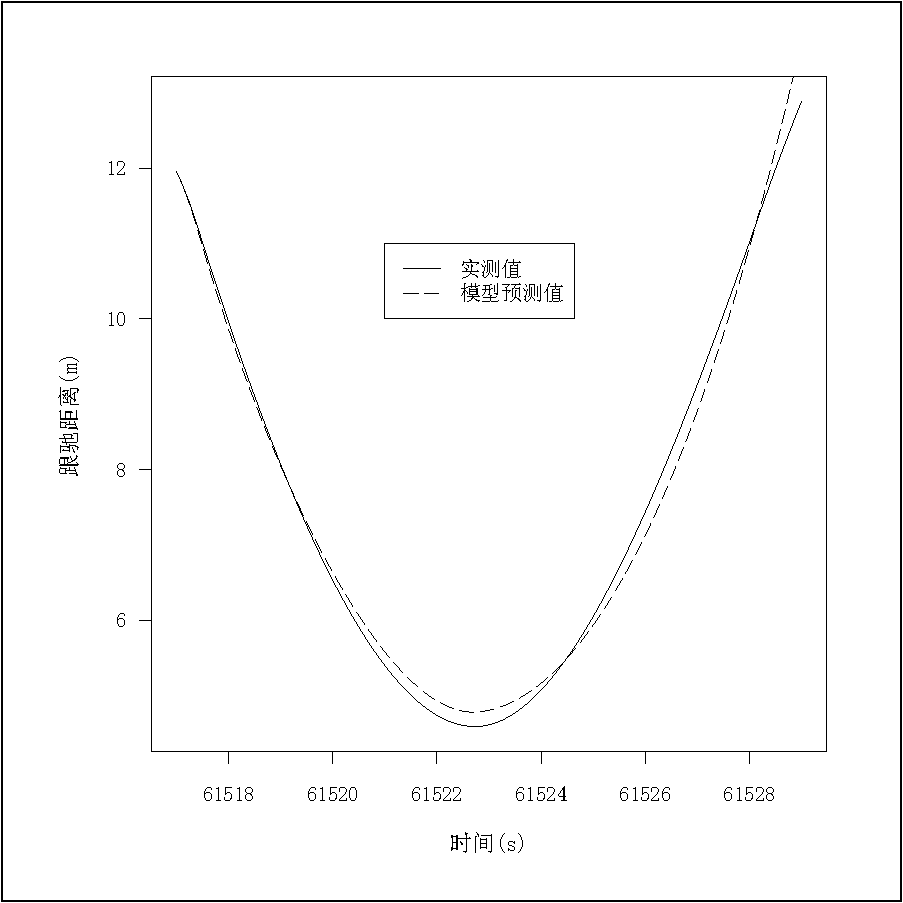
\includegraphics[width=\textwidth]{chapter4-sample-calib-d}
\caption{参数标定结果样例-跟驰距离变化图}
\label{sample-calib-d}
\end{minipage}%
\hspace*{0.04\linewidth}
\begin{minipage}[t]{0.48\linewidth}
\centering
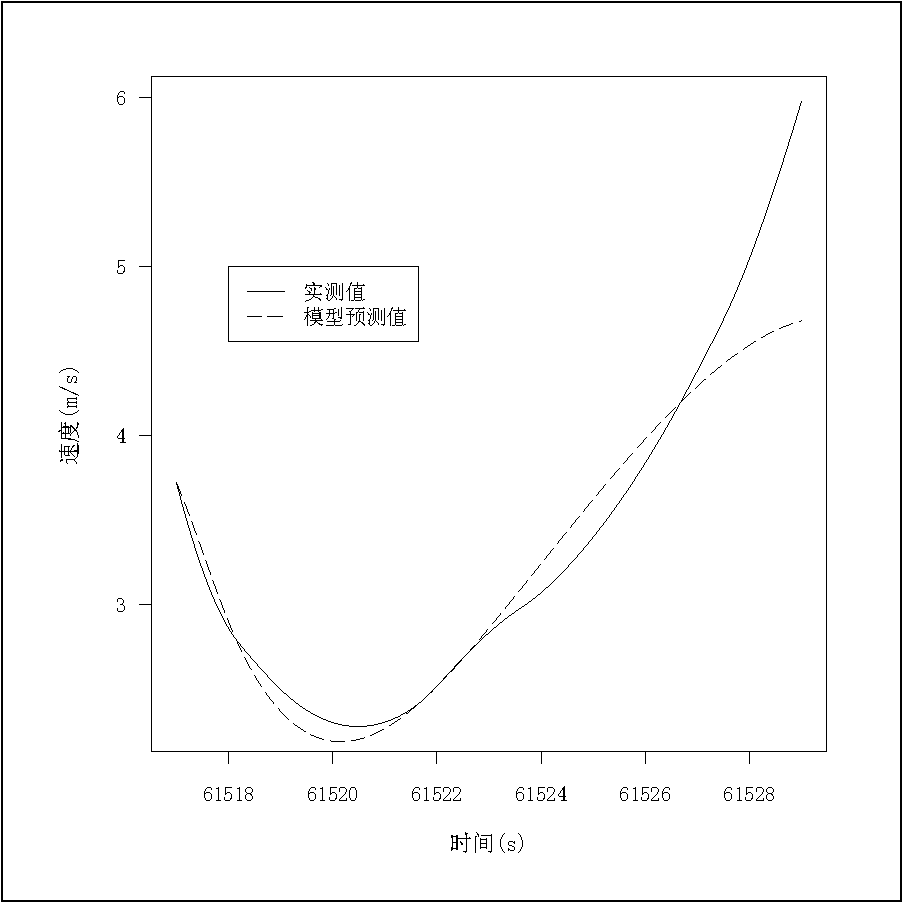
\includegraphics[width=\textwidth]{chapter4-sample-calib-v}
\caption{参数标定结果样例-车速变化图}
\label{sample-calib-v}
\end{minipage}
\end{figure}

% Table generated by Excel2LaTeX from sheet 'calib_result'
\begin{table}[htbp]
  \centering
  \caption{标定参数结果样例}
    \begin{tabular}{rrrrrr}
    \addlinespace
    \toprule
    $DV(m/s)$    & $a_{max}(m/s^2)$    & $b_{max}(m/s^2)$    &  $\Delta X^*(m)$    & $T(s)$ & 目标函数值 \\
    \midrule
    19.10  & 0.62  & 3.42  & 1.20  & 3.90  & 0.02  \\
    9.95  & 0.30  & 0.68  & 4.42  & 4.70  & 0.20  \\
    12.62  & 0.54  & 0.50  & 4.60  & 4.54  & 0.18  \\
    14.00  & 2.88  & 1.00  & 4.80  & 3.99  & 0.46  \\
    1.95  & 0.30  & 5.97  & 1.61  & 4.36  & 0.02  \\
    5.24  & 0.37  & 7.91  & 3.86  & 4.26  & 0.46  \\
    6.28  & 0.63  & 0.53  & 3.44  & 0.84  & 0.13  \\
    2.94  & 2.88  & 0.50  & 4.11  & 3.50  & 0.37  \\
    8.06  & 0.42  & 0.50  & 3.19  & 2.02  & 0.18  \\
    4.19  & 2.04  & 1.80  & 2.37  & 3.15  & 0.23  \\
    21.00  & 0.87  & 9.01  & 0.30  & 3.64  & 0.12  \\
    ...  & ...  & ... & ...  & ...  & ...  \\
    \bottomrule
    \end{tabular}%
  \label{sample-calib-table}%
\end{table}%

%% Table generated by Excel2LaTeX from sheet 'calib_result'
%\begin{table}[htbp]
%  \centering
%  \caption{Add caption}
%    \begin{tabular}{rrrrrrr}
%    \addlinespace
%    \toprule
%    序号    & 参数1   & 参数2   & 参数3   & 参数4   & 参数5   & 目标函数值 \\
%    \midrule
%    1     & 0.0760  & 0.7399  & 6.0596  & 4.9949  & 19.9735  & 0.0523  \\
%    2     & 1.2352  & 0.4298  & 0.5000  & 2.7482  & 5.5988  & 0.0302  \\
%    3     & 1.4037  & 0.5716  & 0.7723  & 2.8879  & 15.5550  & 0.1082  \\
%    4     & 1.9631  & 0.7525  & 2.5320  & 3.1079  & 13.1612  & 0.1056  \\
%    5     & 2.3227  & 0.9399  & 0.5108  & 3.7085  & 8.8214  & 0.1297  \\
%    6     & 13.8583  & 0.3000  & 0.5003  & 0.5603  & 20.0000  & 0.3148  \\
%    7     & 16.9795  & 0.3000  & 0.5000  & 0.6026  & 20.0000  & 0.3120  \\
%    8     & 13.3178  & 0.3067  & 0.5000  & 3.6540  & 6.9455  & 0.7914  \\
%    9     & 1.1541  & 0.4485  & 9.3143  & 2.4454  & 17.8628  & 0.1342  \\
%    10    & 29.4136  & 0.3000  & 0.5000  & 0.3814  & 20.0000  & 0.8865  \\
%    11    & 1.2205  & 0.3000  & 0.5006  & 1.9076  & 17.7410  & 0.4417  \\
%    12    & 14.0335  & 0.3000  & 0.5002  & 0.4269  & 20.0000  & 0.2779  \\
%    13    & 0.0086  & 0.3187  & 8.2771  & 1.8356  & 2.3186  & 0.0137  \\
%    14    & 13.9797  & 0.3000  & 0.5000  & 0.9117  & 20.0000  & 0.5047  \\
%    15    & 14.8697  & 0.3000  & 0.5002  & 0.7457  & 20.0000  & 0.3022  \\
%    16    & 11.6980  & 2.0517  & 1.0119  & 1.8404  & 3.0476  & 0.1829  \\
%    17    & 2.1580  & 0.3000  & 9.0604  & 4.9944  & 19.9765  & 0.1471  \\
%    ...    & ... & ... & ...  & ...  & ...  & ... \\
%    \bottomrule
%    \end{tabular}%
%  \label{tab:addlabel}%
%\end{table}%





\subsection{所得估计参数的可靠程度}

由于车辆轨迹包含的信息不同,因此一段轨迹只能可靠的估计若干个参数,例如一段停车的轨迹是不可能准确地估计出期望车速,最大舒适加速度和最大舒适减速度的参数,却可能很好地估计出停车间距的参数。而加速过程的轨迹则很难估计最大舒适减速度的参数,反之亦然。所以需要估计所得参数的可靠程度。Greene(2000)\cite{Greene2000}指出对于一个变量的点估计其方差至少不小于Cramer-Rao下限,并且指出其值可用对数似然函数在最大似然估计点的二次偏导数估计。Ossen(2008)\cite{Ossen2008}据此提出了使用参数估计点的目标函数二次偏导数来估计参数估计的可靠程度,即:

%二次偏导数与m中位数,variance的关系
\begin{equation}
\left.\frac{\partial^2 g(y_n,\hat{z}_n)}{\partial\beta_i^2}\right| _{\beta_i=\beta_i^*}
\end{equation}

可以理解二次偏导数为估计参数的敏感度,若二次偏导数越大,则不论向任何一个方向一个小的扰动均会造成目标函数值g越大的增加,也就代表参数估计越可靠。

由于所估计参数的取值范围不同,为了统一比较各参数的可靠程度,需对各参数除以其中位数进行规格化,然后计算其二次偏导数。






\subsection{Bootstrap与置信区间估计}
为了得到两组各参数有效的估计,本文中选取目标函数g值0.2以下,并且参数二次偏导数不小于20(则规格化参数改变0.1,目标函数的改变量应在$20\times 0.1^2=0.2$的数量级)的参数估计作为最后的结果进行分析。最终,各参数估计值的分布情况如\autoref{weighted-distr-np1}至\autoref{weighted-distr-pp5}。

% \autoref{weighted-distr-np1},\autoref{weighted-distr-pp1},\autoref{weighted-distr-np2},\autoref{weighted-distr-pp2},\autoref{weighted-distr-np3},\autoref{weighted-distr-pp3},\autoref{weighted-distr-np4},\autoref{weighted-distr-pp4},\autoref{weighted-distr-np5},\autoref{weighted-distr-pp5}

\begin{figure}[htbp]
\begin{minipage}[t]{0.225\linewidth}
\centering
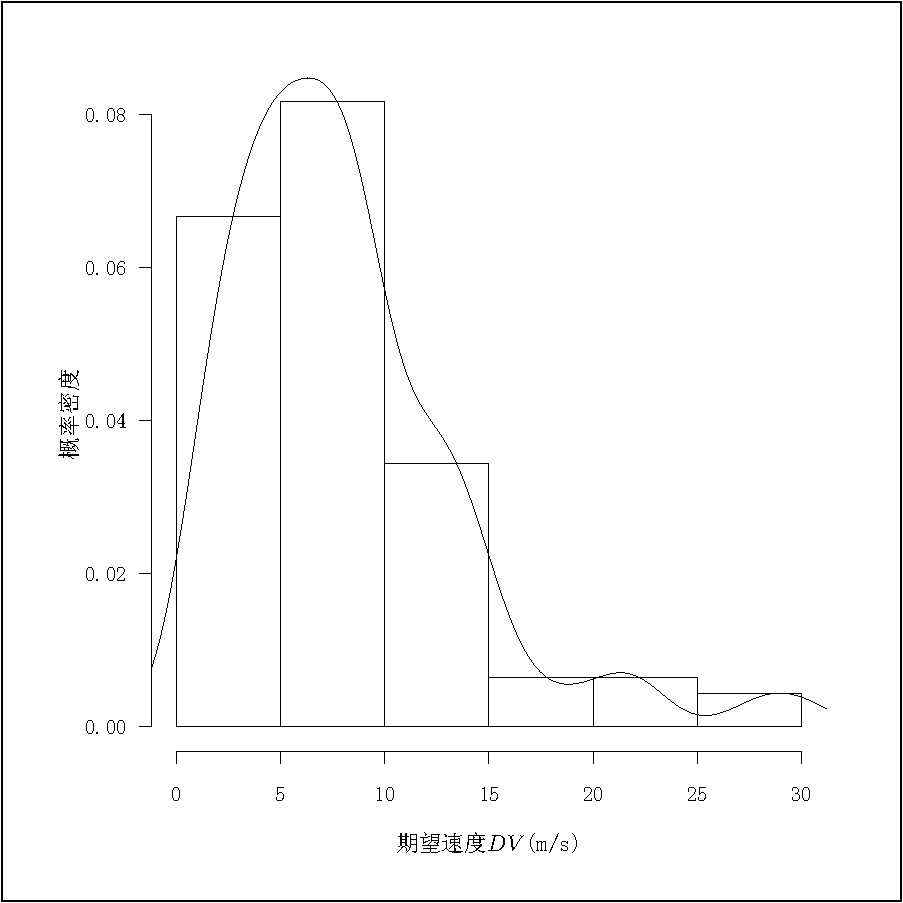
\includegraphics[width=\textwidth]{chapter4-weighted-distr-np1}
\caption{非专业期望速度$DV$分布}
\label{weighted-distr-np1}
\end{minipage}%
\hspace*{0.03\linewidth}
\begin{minipage}[t]{0.225\linewidth}
\centering
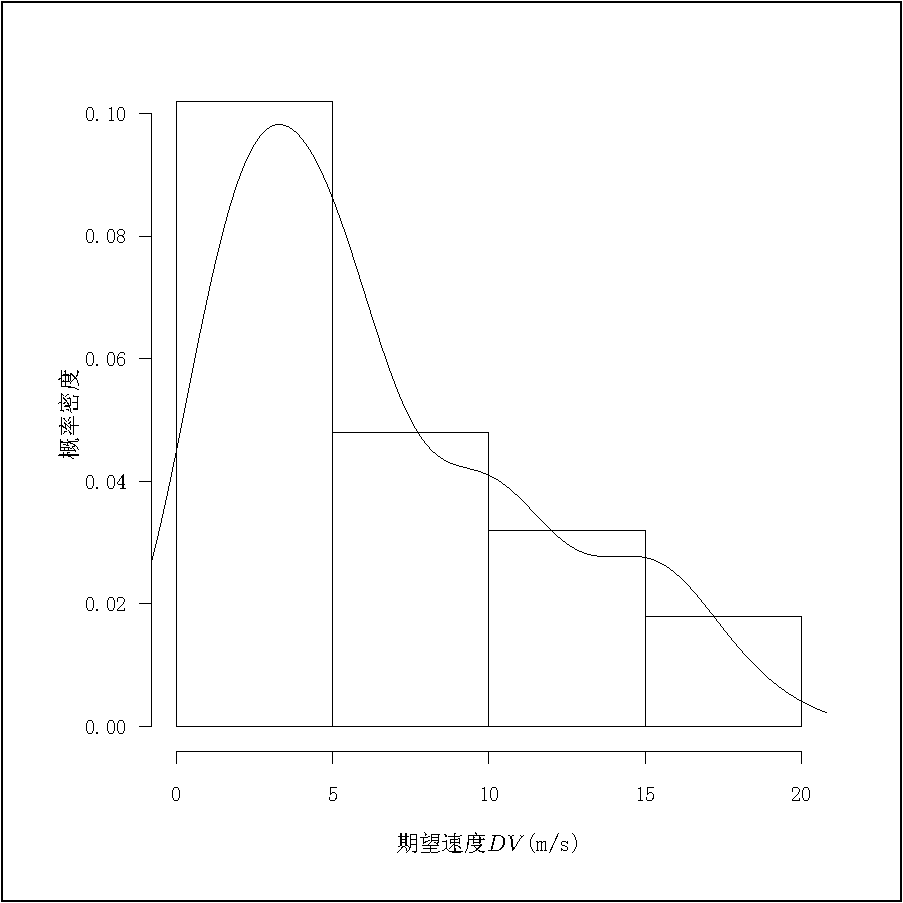
\includegraphics[width=\textwidth]{chapter4-weighted-distr-pp1}
\caption{专业期望速度$DV$分布}
\label{weighted-distr-pp1}
\end{minipage}
\hspace*{0.03\linewidth}
\begin{minipage}[t]{0.225\linewidth}
\centering
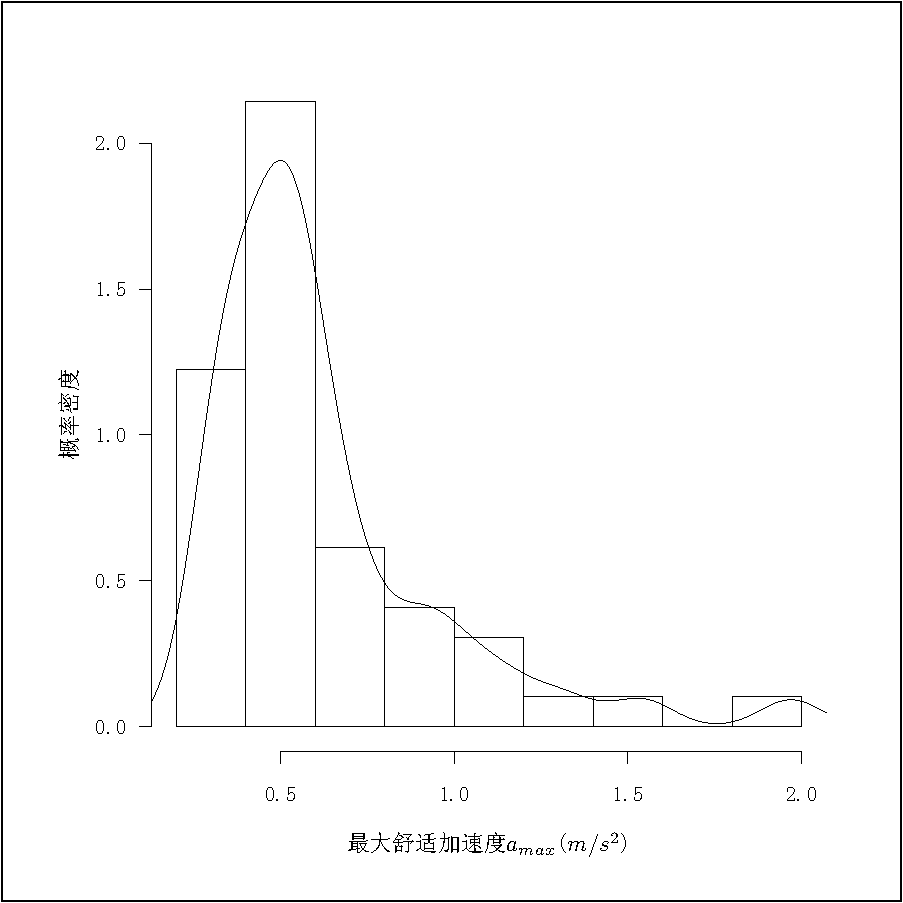
\includegraphics[width=\textwidth]{chapter4-weighted-distr-np2}
\caption{非专业最大舒适加速度$a_{max}$分布}
\label{weighted-distr-np2}
\end{minipage}%
\hspace*{0.03\linewidth}
\begin{minipage}[t]{0.225\linewidth}
\centering
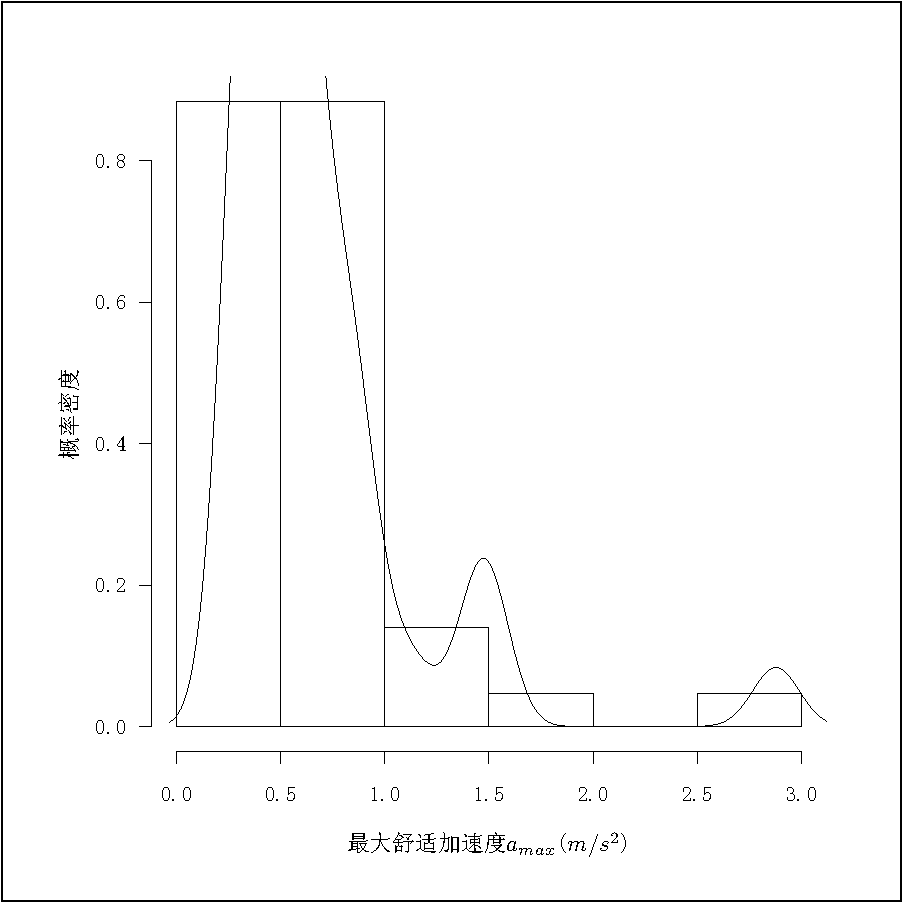
\includegraphics[width=\textwidth]{chapter4-weighted-distr-pp2}
\caption{专业最大舒适加速度$a_{max}$分布}
\label{weighted-distr-pp2}
\end{minipage}
\begin{minipage}[t]{0.225\linewidth}
\centering
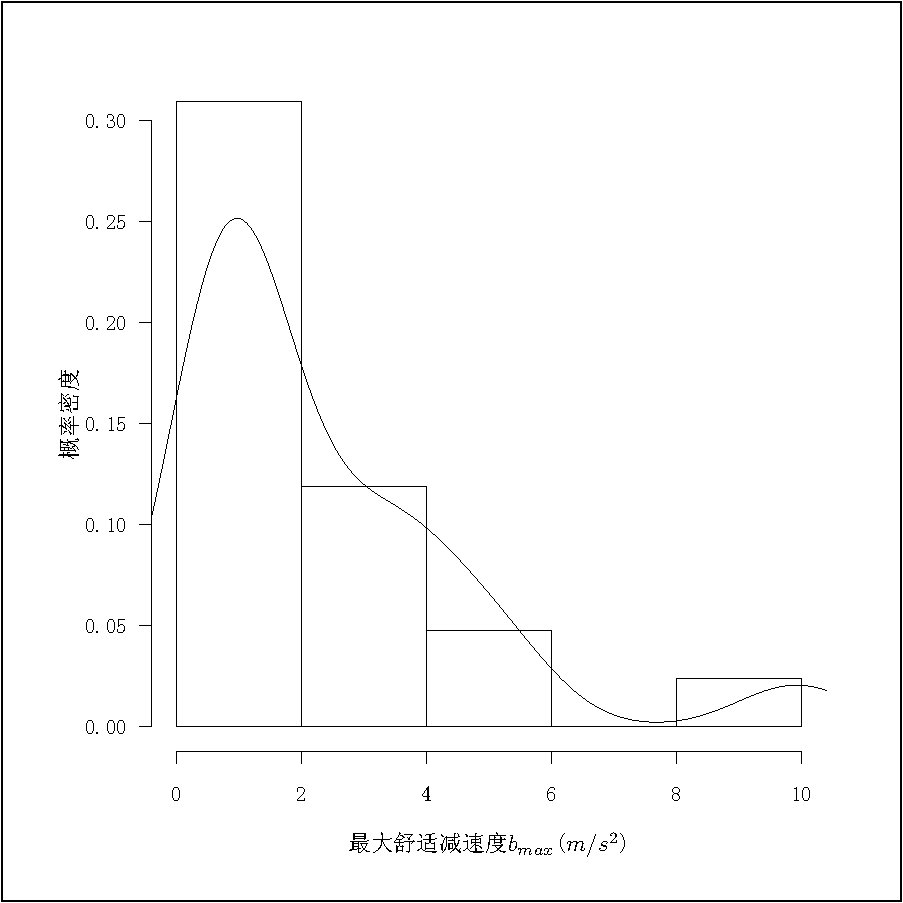
\includegraphics[width=\textwidth]{chapter4-weighted-distr-np3}
\caption{非专业最大舒适减速度$b_{max}$分布}
\label{weighted-distr-np3}
\end{minipage}%
\hspace*{0.03\linewidth}
\begin{minipage}[t]{0.225\linewidth}
\centering
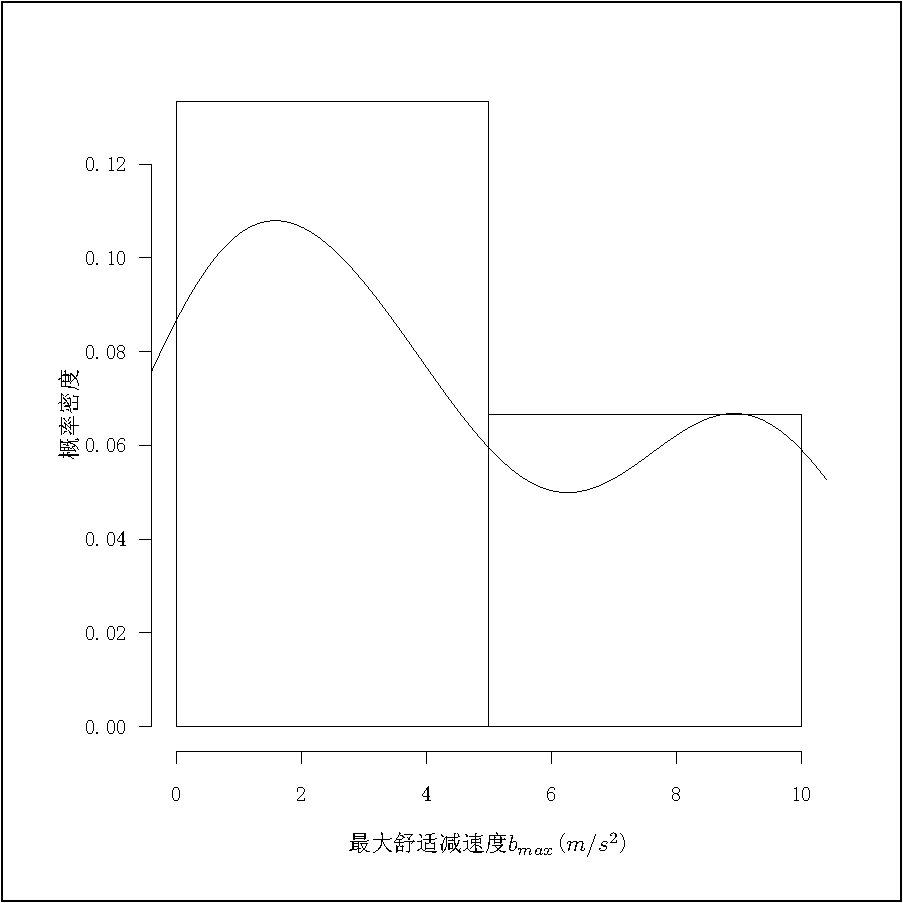
\includegraphics[width=\textwidth]{chapter4-weighted-distr-pp3}
\caption{专业最大舒适减速度$b_{max}$分布}
\label{weighted-distr-pp3}
\end{minipage}
\hspace*{0.03\linewidth}
\begin{minipage}[t]{0.225\linewidth}
\centering
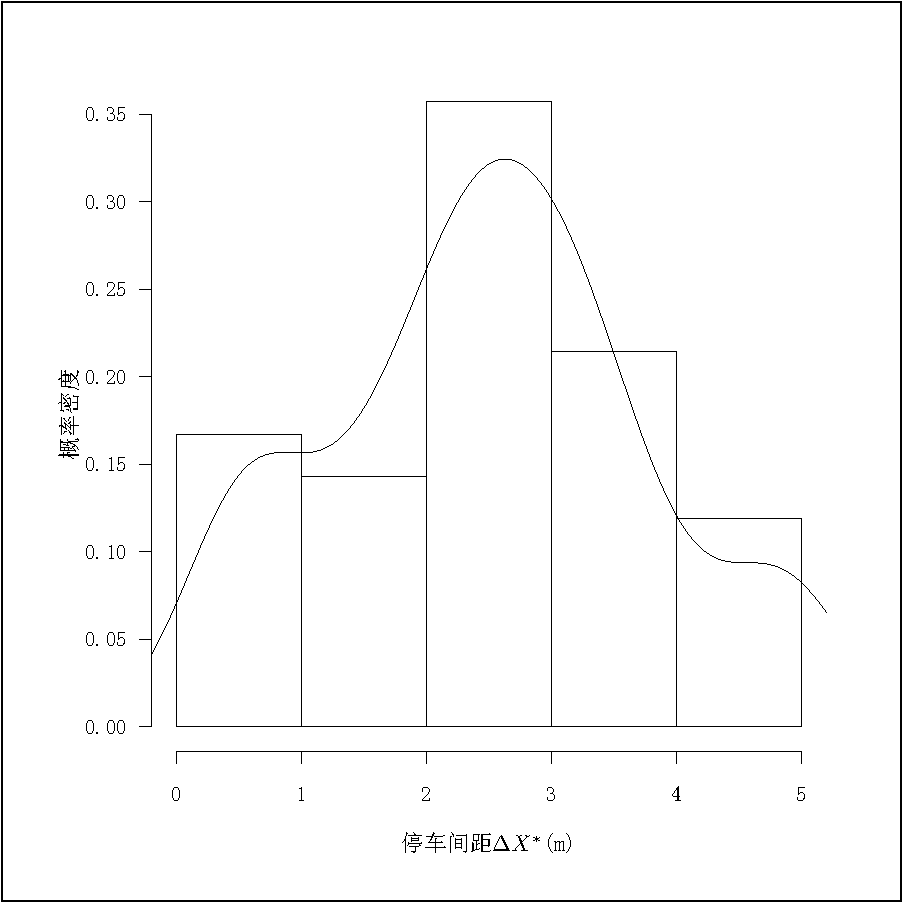
\includegraphics[width=\textwidth]{chapter4-weighted-distr-np4}
\caption{非专业停车间距$\Delta X^*$分布}
\label{weighted-distr-np4}
\end{minipage}%
\hspace*{0.03\linewidth}
\begin{minipage}[t]{0.225\linewidth}
\centering
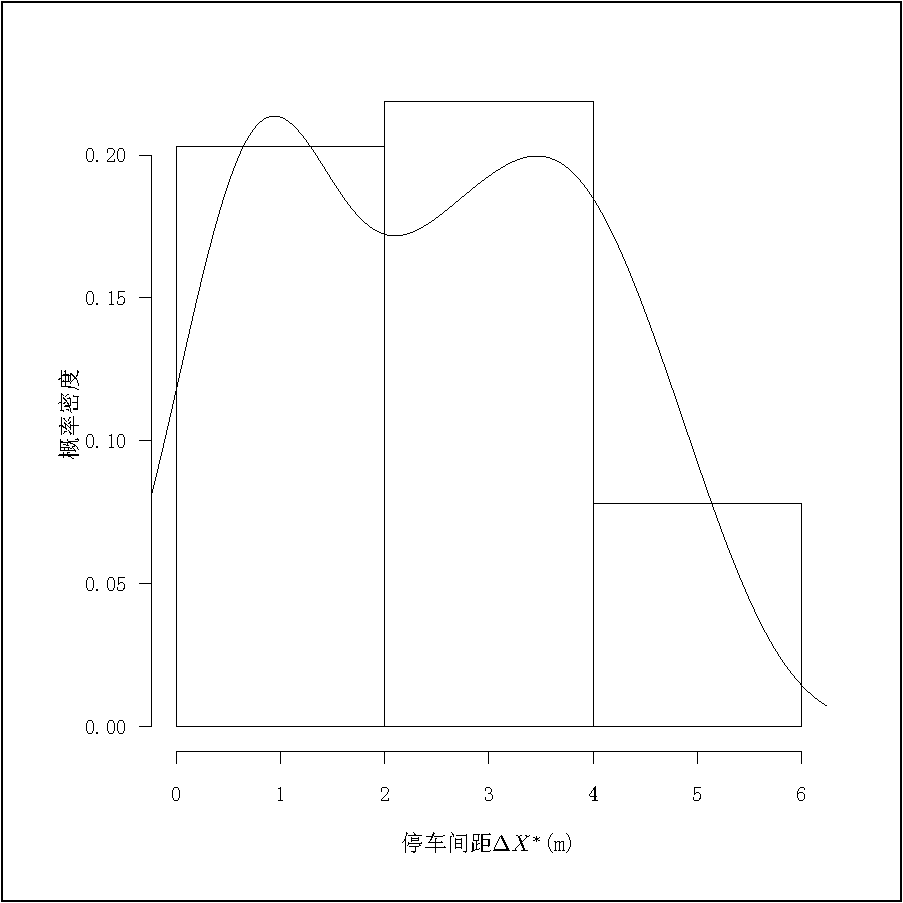
\includegraphics[width=\textwidth]{chapter4-weighted-distr-pp4}
\caption{专业停车间距$\Delta X^*$分布}
\label{weighted-distr-pp4}
\end{minipage}
\begin{minipage}[t]{0.225\linewidth}
\centering
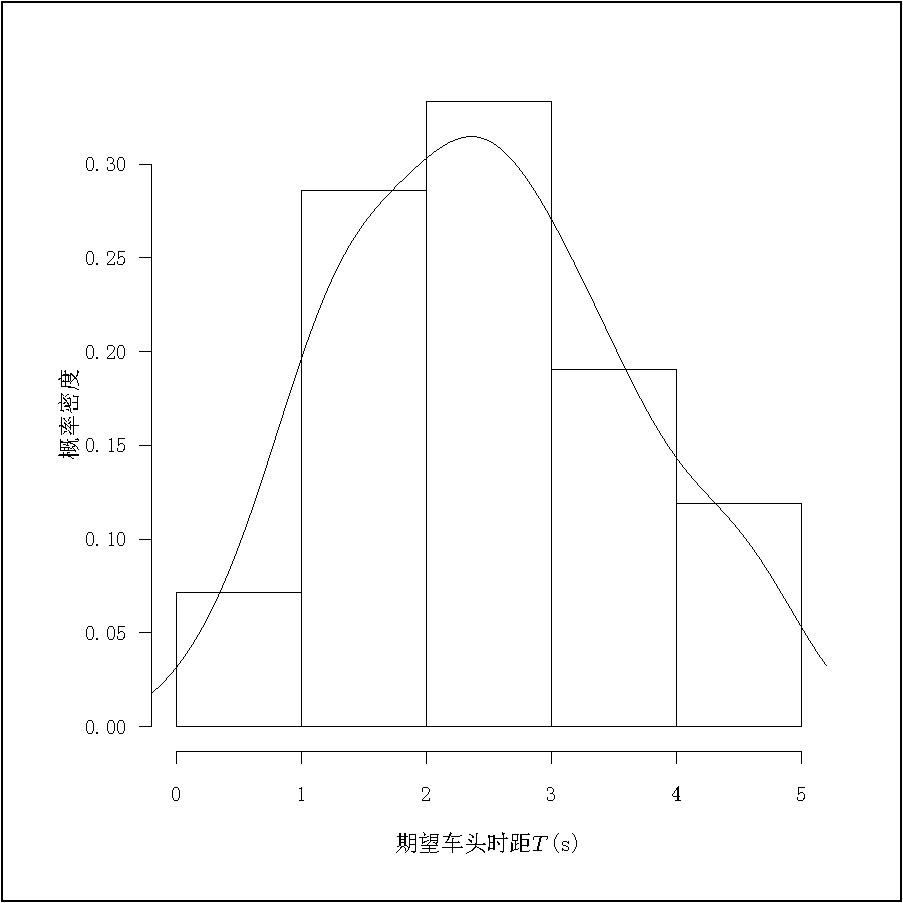
\includegraphics[width=\textwidth]{chapter4-weighted-distr-np5}
\caption{非专业期望车头时距$T$分布}
\label{weighted-distr-np5}
\end{minipage}%
\hspace*{0.03\linewidth}
\begin{minipage}[t]{0.225\linewidth}
\centering
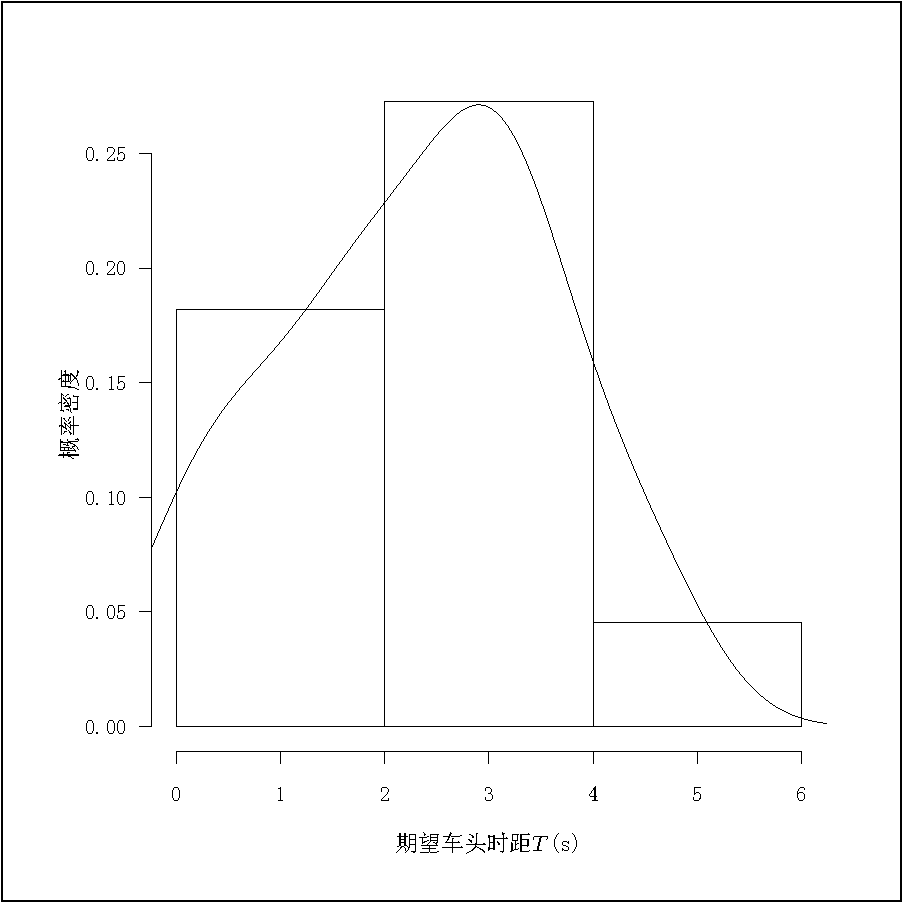
\includegraphics[width=\textwidth]{chapter4-weighted-distr-pp5}
\caption{专业期望车头时距$T$分布}
\label{weighted-distr-pp5}
\end{minipage}
\end{figure}

% \begin{figure}[htbp]
% \begin{minipage}[t]{0.48\linewidth}
% \centering
% 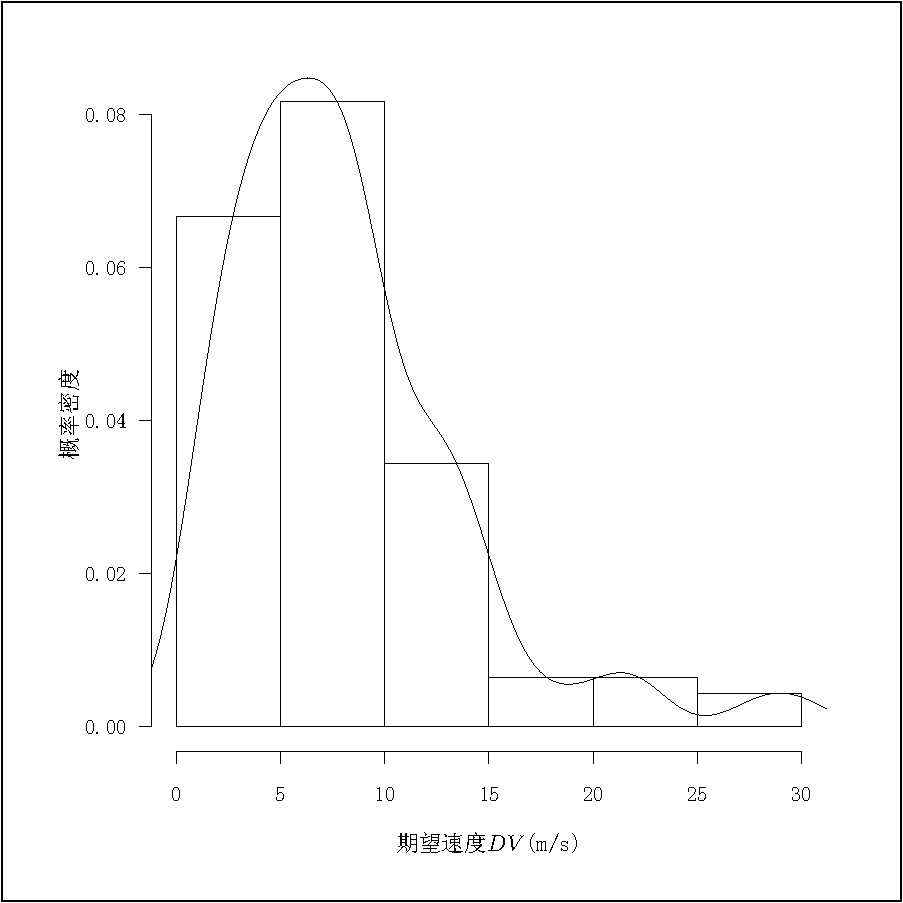
\includegraphics[width=\textwidth]{chapter4-weighted-distr-np1}
% \caption{非专业期望速度$DV$分布}
% \label{weighted-distr-np1}
% \end{minipage}%
% \hspace*{0.04\linewidth}
% \begin{minipage}[t]{0.48\linewidth}
% \centering
% 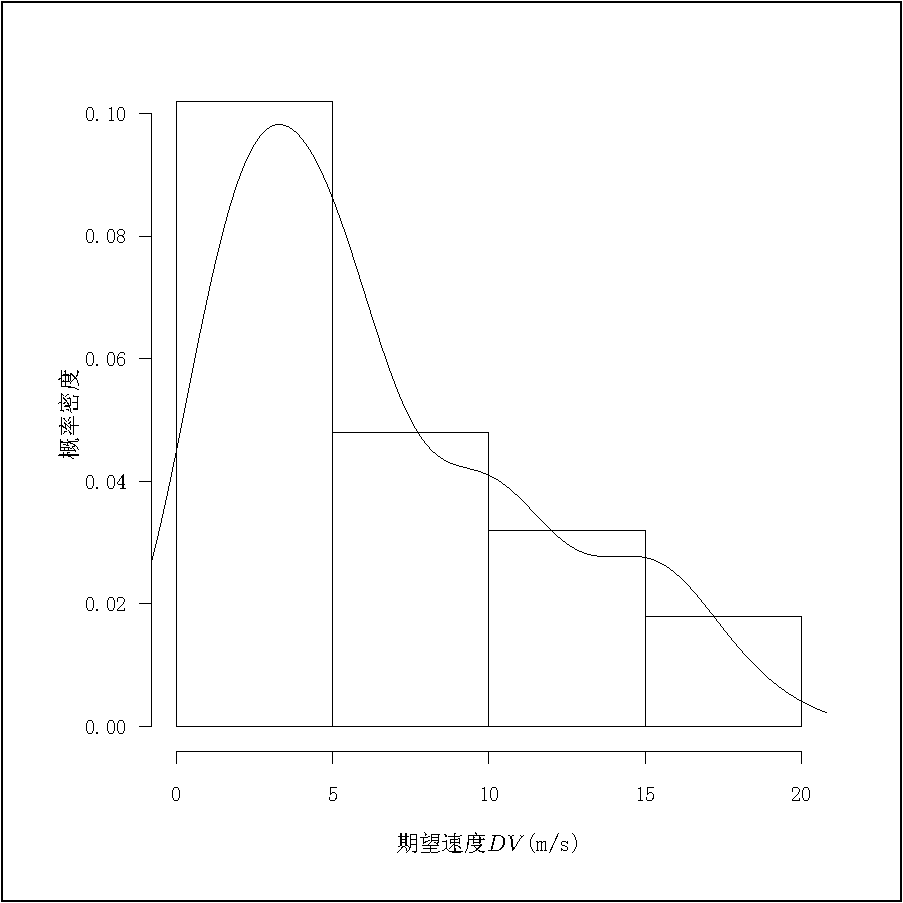
\includegraphics[width=\textwidth]{chapter4-weighted-distr-pp1}
% \caption{专业期望速度$DV$分布}
% \label{weighted-distr-pp1}
% \end{minipage}
% \end{figure}

% \begin{figure}[htbp]
% \begin{minipage}[t]{0.48\linewidth}
% \centering
% 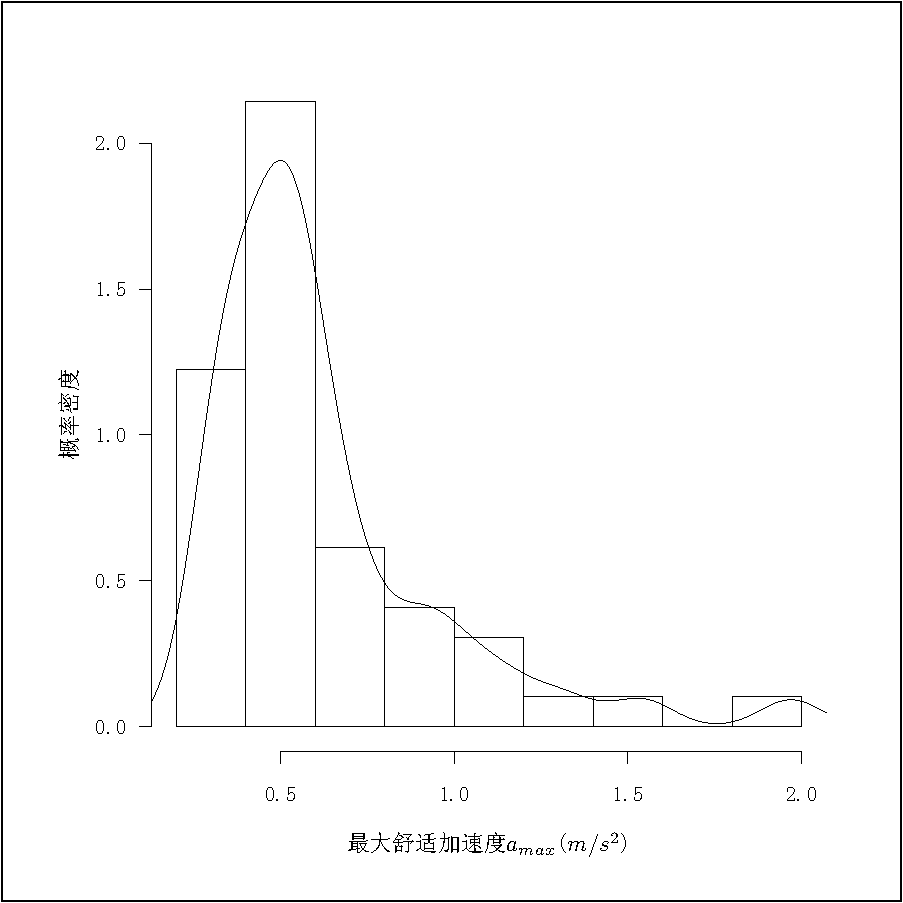
\includegraphics[width=\textwidth]{chapter4-weighted-distr-np2}
% \caption{非专业最大舒适加速度$a_{max}$分布}
% \label{weighted-distr-np2}
% \end{minipage}%
% \hspace*{0.04\linewidth}
% \begin{minipage}[t]{0.48\linewidth}
% \centering
% 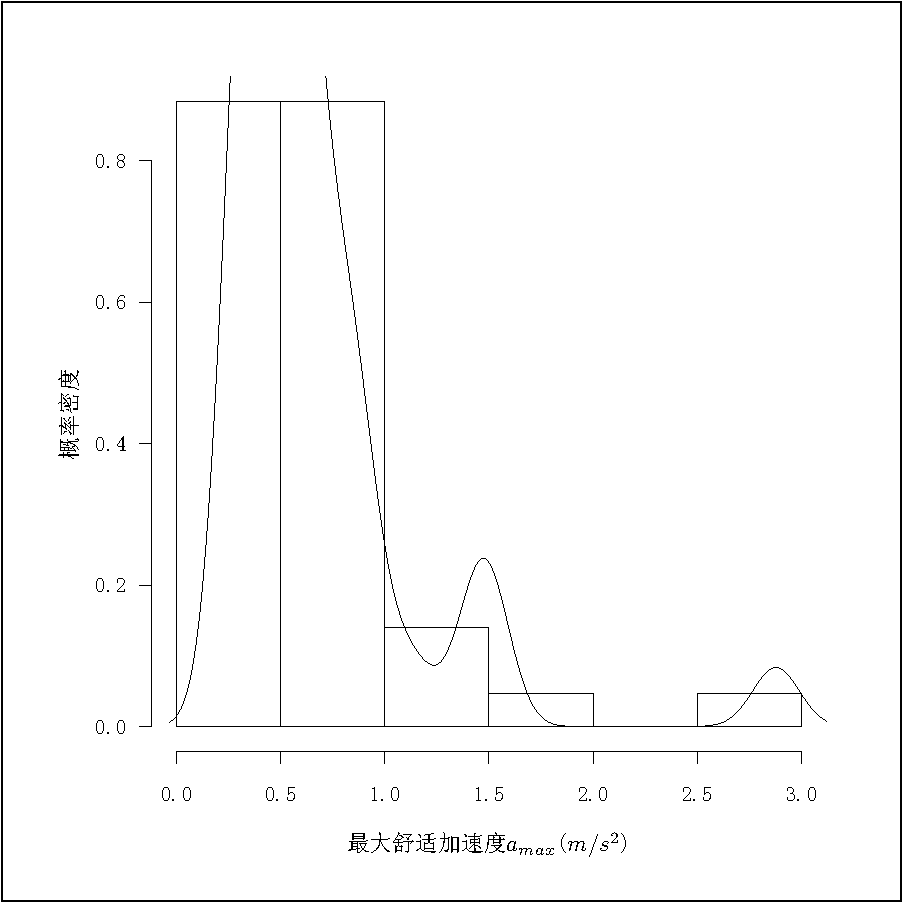
\includegraphics[width=\textwidth]{chapter4-weighted-distr-pp2}
% \caption{专业最大舒适加速度$a_{max}$分布}
% \label{weighted-distr-pp2}
% \end{minipage}
% \end{figure}

% \begin{figure}[htbp]
% \begin{minipage}[t]{0.48\linewidth}
% \centering
% 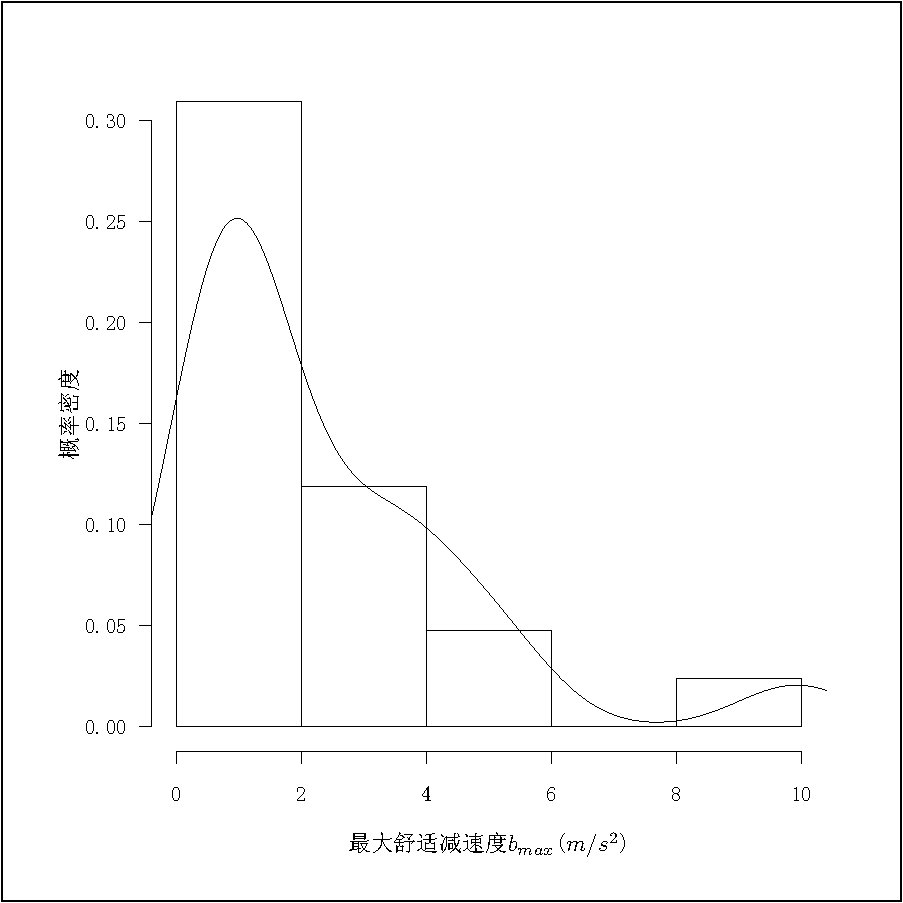
\includegraphics[width=\textwidth]{chapter4-weighted-distr-np3}
% \caption{非专业最大舒适减速度$b_{max}$分布}
% \label{weighted-distr-np3}
% \end{minipage}%
% \hspace*{0.04\linewidth}
% \begin{minipage}[t]{0.48\linewidth}
% \centering
% 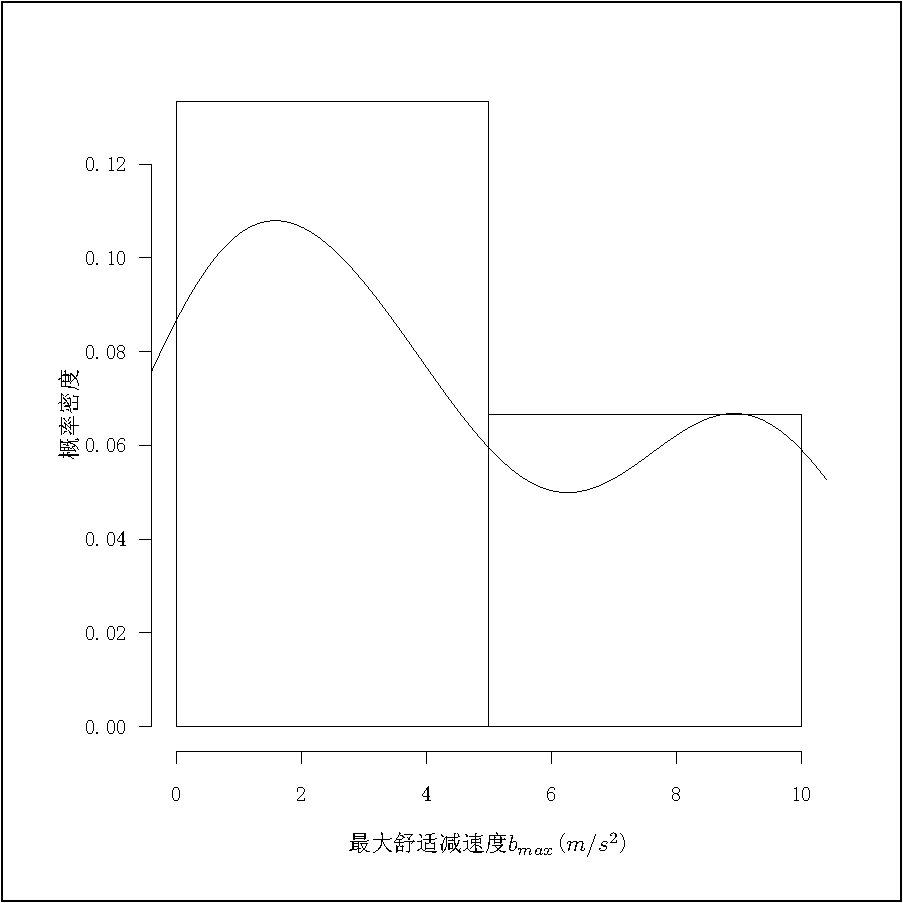
\includegraphics[width=\textwidth]{chapter4-weighted-distr-pp3}
% \caption{专业最大舒适减速度$b_{max}$分布}
% \label{weighted-distr-pp3}
% \end{minipage}
% \end{figure}

% \begin{figure}[htbp]
% \begin{minipage}[t]{0.48\linewidth}
% \centering
% 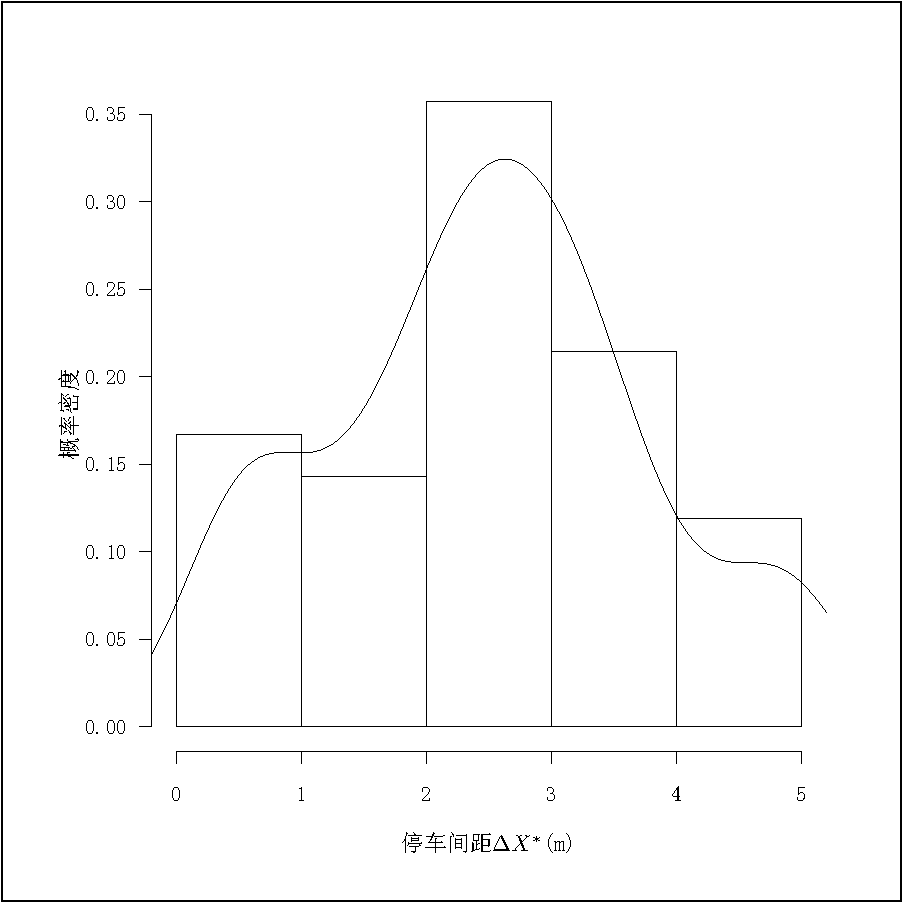
\includegraphics[width=\textwidth]{chapter4-weighted-distr-np4}
% \caption{非专业停车间距$\Delta X^*$分布}
% \label{weighted-distr-np4}
% \end{minipage}%
% \hspace*{0.04\linewidth}
% \begin{minipage}[t]{0.48\linewidth}
% \centering
% 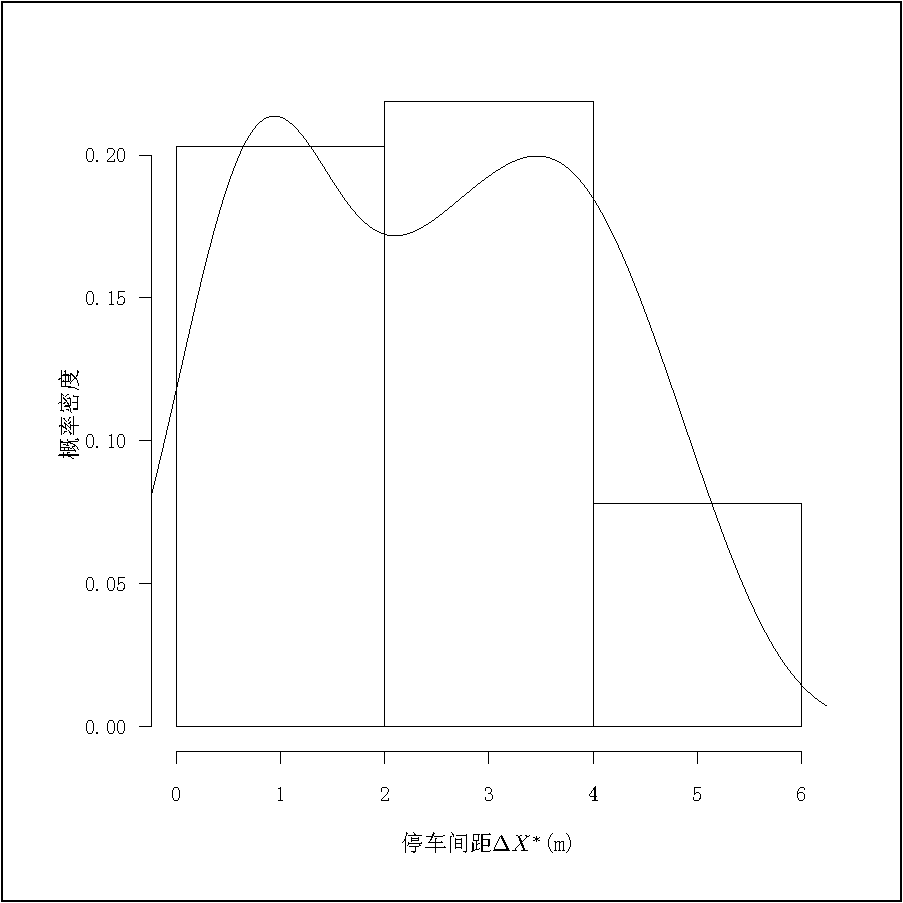
\includegraphics[width=\textwidth]{chapter4-weighted-distr-pp4}
% \caption{专业停车间距$\Delta X^*$分布}
% \label{weighted-distr-pp4}
% \end{minipage}
% \end{figure}

% \begin{figure}[htbp]
% \begin{minipage}[t]{0.48\linewidth}
% \centering
% 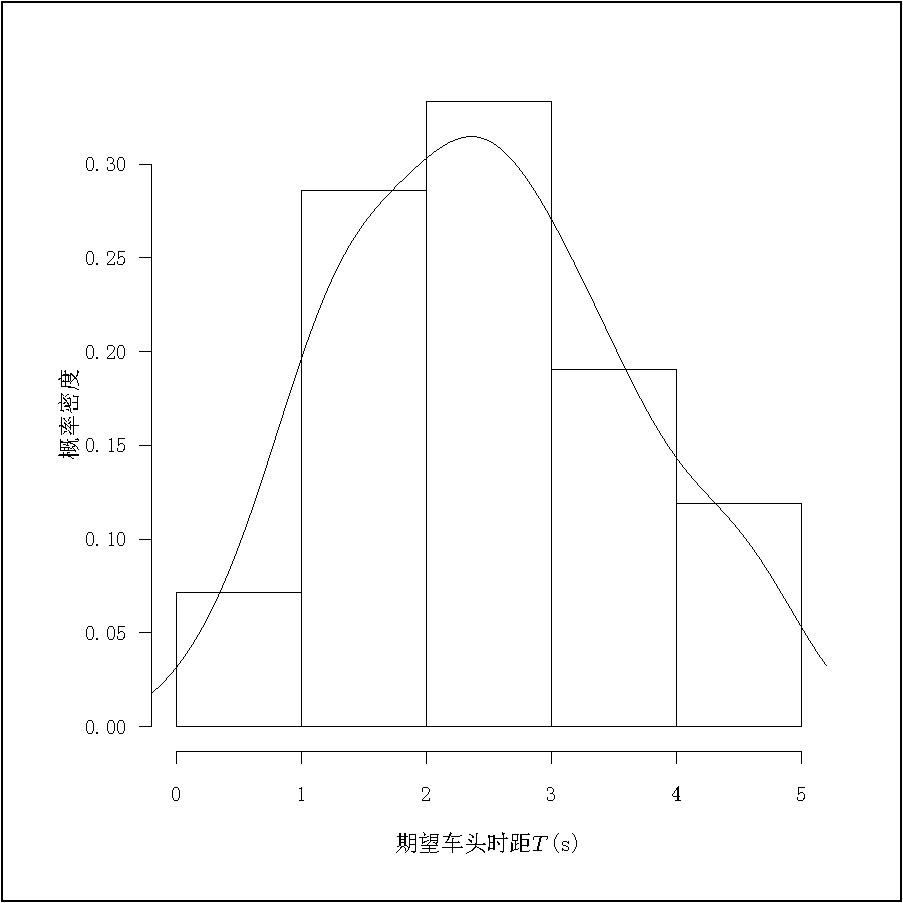
\includegraphics[width=\textwidth]{chapter4-weighted-distr-np5}
% \caption{非专业期望车头时距$T$分布}
% \label{weighted-distr-np5}
% \end{minipage}%
% \hspace*{0.04\linewidth}
% \begin{minipage}[t]{0.48\linewidth}
% \centering
% 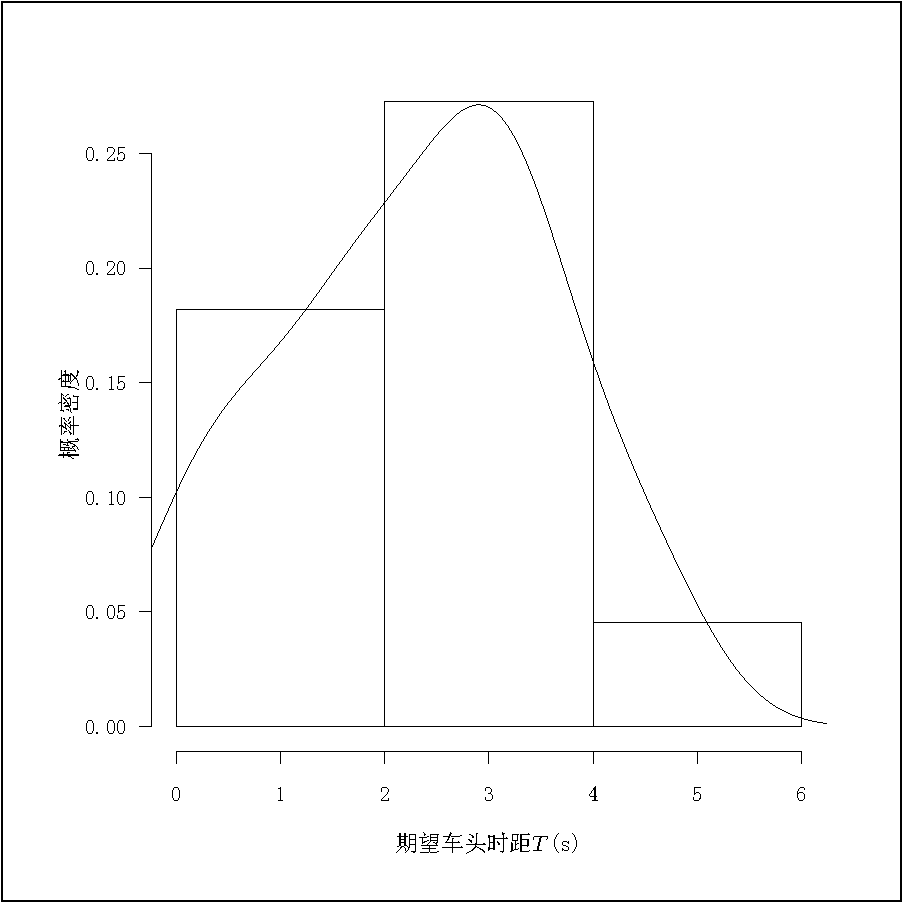
\includegraphics[width=\textwidth]{chapter4-weighted-distr-pp5}
% \caption{专业期望车头时距$T$分布}
% \label{weighted-distr-pp5}
% \end{minipage}
% \end{figure}

由图中可以明显看出各参数的样本分布均不符合正态分布,为了得到各参数在总体中的有效估计,并且比较两组驾驶人各参数的异同。本文使用Bootstrap,也称自助法来根据样本数据估计各参数的置信区间。
%bootstrap介绍
%bootstrapping is a computer-based method for assigning measures of accuracy to sample estimates (Efron and Tibshirani 1994). This technique allows estimation of the sample distribution of almost any statistic using only very simple methods (Varian 2005).
Efron(1979)\cite{Efron1979}最早明确提出了Bootstrap方法。Bootstrap方法是非参数统计中一种重要的估计统计量方差进而进行区间估计的统计方法。其核心思想是通过对样本大量(N一般不小于1000)的可重复的重抽样,通过计算重抽样样本的统计量构造Bootstrap分布来近似总体的抽样分布,从而估计样本所属总体的统计量。其渐进有效性对大多数常用分布和统计量已被证明。使用Bootstrap方法主要的优点在于无需对总体的分布进行假设,只需样本中的个体满足独立同分布的条件,便能对总体的统计量(例如均值)进行有效的估计。

对于本文中的数据,相邻轨迹数据的间隔一般都在10s以上。基于驾驶人自身行为具有差异性的假设,可以认为驾驶人在不同时刻的驾驶行为是独立的,那么估计所得各参数值可以认为符合独立同分布的条件。

% an independent and identically distributed population,this can be implemented by constructing a number of resamples of the observed dataset (and of equal size to the observed dataset), each of which is obtained by random sampling with replacement from the original dataset.
%   (1) 采用重抽样技术从原始样本中抽取一定数量(自己给定)的样本,此过程允许重复抽样。   (2) 根据抽出的样本计算给定的统计量T。   (3) 重复上述N次(一般大于1000),得到N个统计量T。   (4) 计算上述N各统计量T的样本方差,得到统计量的方差。

Bootstrap结果中样本均值与总体均值的95\%置信区间估计如\autoref{boot-mean},样本标准差与总体标准差的95\%置信区间估计如\autoref{boot-mean}。Kesting和Treiber(2008)\cite{Kesting2008}的对照结果如\autoref{reference-idm}。可以发现各参数均值均在合理范围内,且非专业组与专业组的参数均值主要在期望速度$DV(m/s)$和最大舒适减速度$b_{max}(m/s^2)$存在差异。

\begin{table}[htbp]
  \centering
  \caption{IDM参数均值估计}
    \begin{tabular}{rrrrr}
    \addlinespace
    \toprule
          & \multicolumn{ 2}{c}{非专业驾驶人} & \multicolumn{ 2}{c}{专业驾驶人} \\
    \midrule
          & 样本均值  & 95\%置信区间 & 样本均值  & 95\%置信区间 \\
    $DV(m/s)$ & 8.09  & (6.978,9.236) & 6.48  & (5.549,7.421) \\
    $a_{max}(m/s^2)$ & 0.63  & (0.531,0.718) & 0.66  & (0.523,0.802) \\
    $b_{max}(m/s^2)$ & 2.33  & (1.362,3.295) & 4.29  & (2.621,5.949) \\
    $\Delta X^*(m)$     & 2.50  & (2.124,2.878) & 2.41  & (1.905,2.931) \\
    $T(s)$     & 2.46  & (2.140,2.783) & 2.34  & (1.810,2.886) \\
    \bottomrule
    \end{tabular}%
  \label{boot-mean}%
\end{table}%

% Table generated by Excel2LaTeX from sheet 'Sheet1'
\begin{table}[htbp]
  \centering
  \caption{IDM参数标准差估计}
    \begin{tabular}{rrrrr}
    \addlinespace
    \toprule
          & \multicolumn{ 2}{c}{非专业驾驶人} & \multicolumn{ 2}{c}{专业驾驶人} \\
    \midrule
          & 样本标准差 & 95\%置信区间 & 样本标准差 & 95\%置信区间 \\
    $DV(m/s)$ & 5.55  & (4.338,6.866) & 4.83  & (4.286,5.440) \\
    $a_{max}(m/s^2)$ & 0.34  & (0.229,0.474) & 0.46  & (0.243,0.724) \\
    $b_{max}(m/s^2)$ & 2.31  & (1.310,3.531) & 3.69  & (3.053,4.593) \\
    $\Delta X^*(m)$    & 1.27  & (1.043,1.523) & 1.50  & (1.305,1.749) \\
    $T(s)$      & 1.12  & (0.936,1.333) & 1.32  & (1.052,1.643) \\
    \bottomrule
    \end{tabular}%
  \label{boot-sd}%
\end{table}%

% Table generated by Excel2LaTeX from sheet 'Sheet1'
\begin{table}[htbp]
  \centering
  \caption{Kesting\cite{Kesting2008}的IDM参数估计}
    \begin{tabular}{rrrr}
    \addlinespace
    \toprule
          & \multicolumn{ 3}{c}{Data Set1} \\
    \midrule
          & $F_{rel}(s)$ & $F_{mix}(s)$ & $F_{abs}(s)$ \\
    误差(\%)     & 24.0  & 20.7  & 20.7  \\
    $DV(m/s)$    & 70.0  & 69.9  & 70.0  \\
    $T(s)$    & 1.07  & 1.12  & 1.03  \\
    $\Delta X^*(m)$    & 2.41  & 2.33  & 2.56  \\
    $a_{max}(m/s^2)$     & 1.00  & 1.23  & 1.40  \\
    $b_{max}(m/s^2)$     & 3.21  & 3.20  & 3.73  \\
    \bottomrule
    \end{tabular}%
  \label{reference-idm}%
\end{table}%
%做均值和SD


对样本的分层Bootstrap,可以获得总体的非专业与专业驾驶人参数均值差的置信区间估计,期望速度$DV(m/s)$和最大舒适减速度$b_{max}(m/s^2)$的Bootstrap分布及正态Q-Q如\autoref{p1-df-qq}和\autoref{p3-df-qq},图中的Bootstrap分布基本上符合正态分布,且样本均值差具有较小的偏差,因此其总体均值差的95\%置信区间是可靠的。置信区间估计结果如\autoref{boot-df},可以看到非专业驾驶人的期望速度大于专业驾驶人,而其最大舒适减速度小于专业驾驶人。

综合以上结果,可以推断在不同的驾驶人之间其期望速度和最大减速度存在差异。期望速度的差异说明驾驶人在大致相同条件下其希望的行驶速度是不同的,这反映了不同驾驶人综合考虑自身需求和对道路交通条件适应的结果。由于样本中非专业组与专业组的年龄存在差异,期望速度的差异可能因为年龄或其他差异而非驾驶经验的差异。而不同驾驶人间最大减速度的差异,反应了驾驶人减速的能力,非专业驾驶人由于驾驶经验较短可能对于潜在的危险情况认识不足,导致其减速能力较低。


% Table generated by Excel2LaTeX from sheet 'Sheet1'
\begin{table}[htbp]
  \centering
  \caption{样本均值差(非专业减去专业)与总体均值差95\%置信区间估计}
    \begin{tabular}{rrr}
    \addlinespace
    \toprule
          & 样本均值差 & 95\%置信区间 \\
    \midrule
    $DV(m/s)$ & 1.60  & (0.072,3.048) \\
    $a_{max}(m/s^2)$ & -0.03  & (-0.204,0.137) \\
    $b_{max}(m/s^2)$ & -1.95  & (-3.774,-0.115) \\
    $\Delta X^*(m)$     & 0.09  & (-0.552,0.751) \\
    $T(s)$     & 0.12  & (-0.519,-0.742) \\
    \bottomrule
    \end{tabular}%
  \label{boot-df}%
\end{table}%

%\begin{figure}[H]
%\begin{center}
%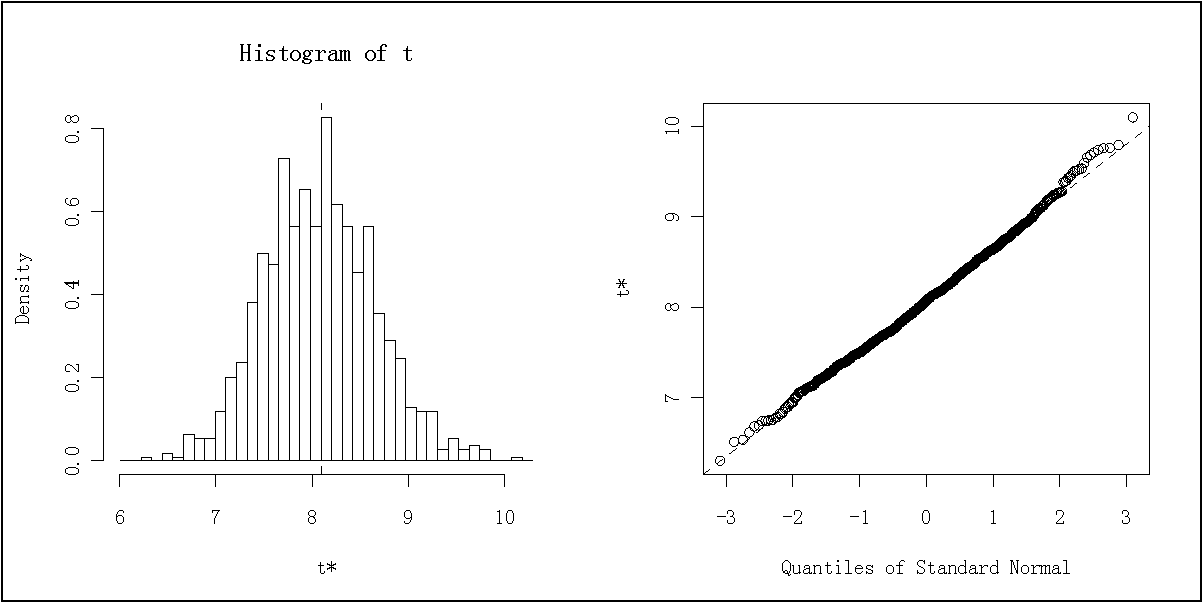
\includegraphics{chapter4-bootstrap-np1-mean.pdf}
%\end{center}
%\caption{非专业驾驶人期望速度$v_{des}$参数Bootstrap分布及正态Q-Q}
%\end{figure}
%
%\begin{figure}[H]
%\begin{center}
%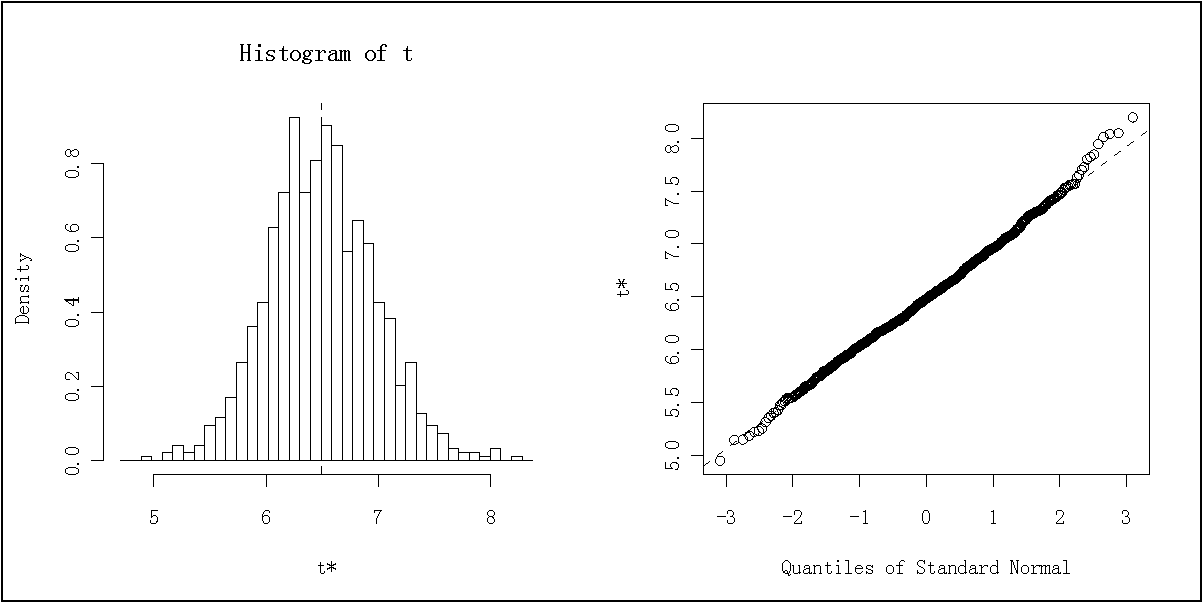
\includegraphics{chapter4-bootstrap-pp1-mean.pdf}
%\end{center}
%\caption{专业驾驶人期望速度$v_{des}$参数Bootstrap分布及正态Q-Q}
%\end{figure}

\begin{figure}[htbp]
\begin{center}
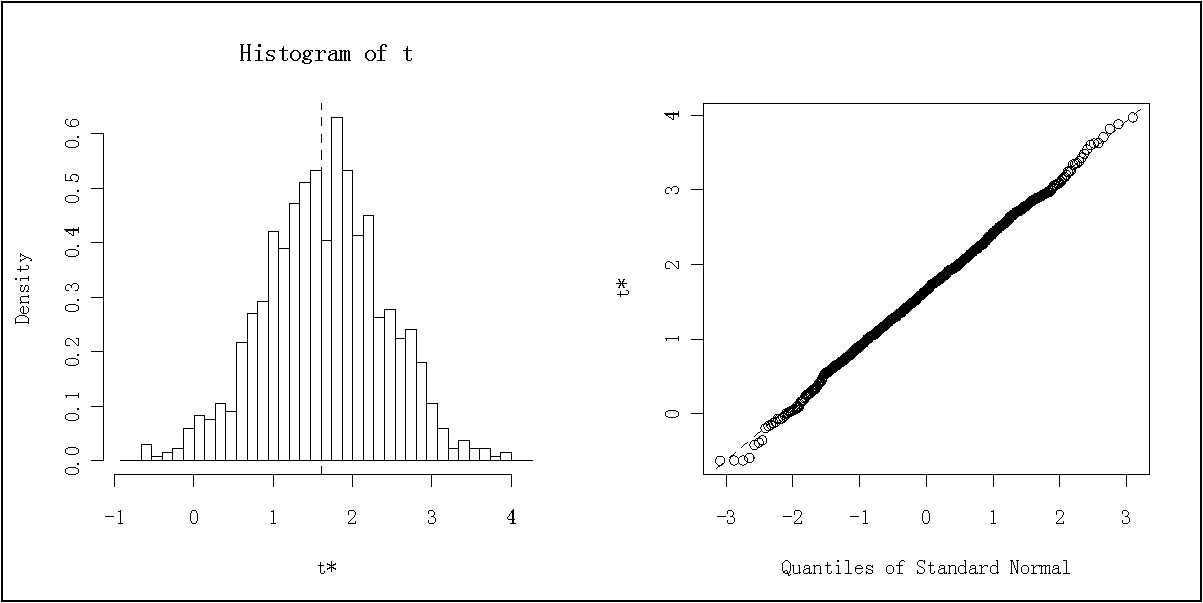
\includegraphics[width=0.6\textwidth]{chapter4-bootstrap-p1df-mean.pdf}
\end{center}
\caption{非专业与专业驾驶人期望速度$v_{des}$参数差值分层Bootstrap分布及正态Q-Q}
\label{p1-df-qq}
\end{figure}





%\begin{figure}[H]
%\begin{center}
%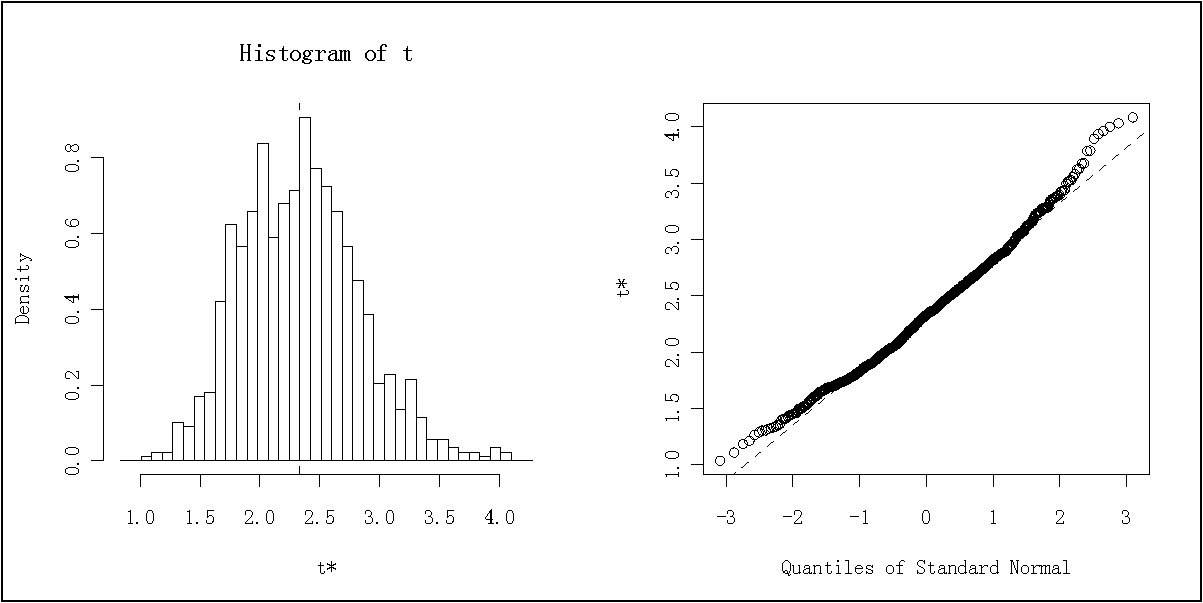
\includegraphics{chapter4-bootstrap-np3-mean.pdf}
%\end{center}
%\caption{非专业驾驶人最大舒适减速度$b_{max}$参数Bootstrap分布及正态Q-Q}
%\end{figure}
%
%\begin{figure}[H]
%\begin{center}
%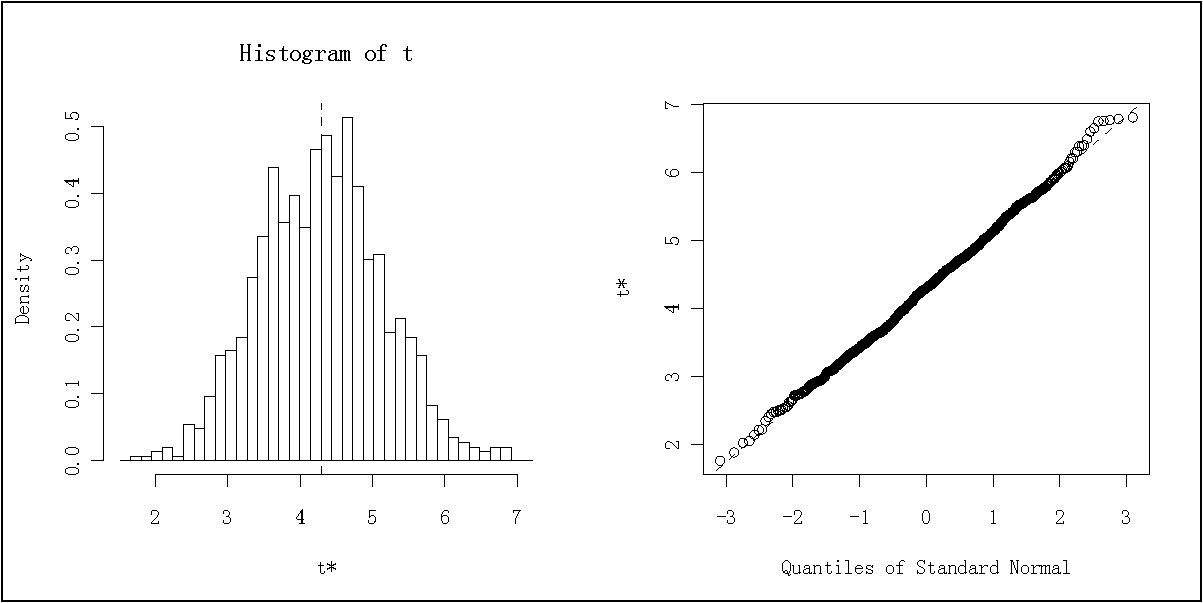
\includegraphics{chapter4-bootstrap-pp3-mean.pdf}
%\end{center}
%\caption{专业驾驶人最大舒适减速度$b_{max}$参数Bootstrap分布及正态Q-Q}
%\end{figure}

\begin{figure}[htbp]
\begin{center}
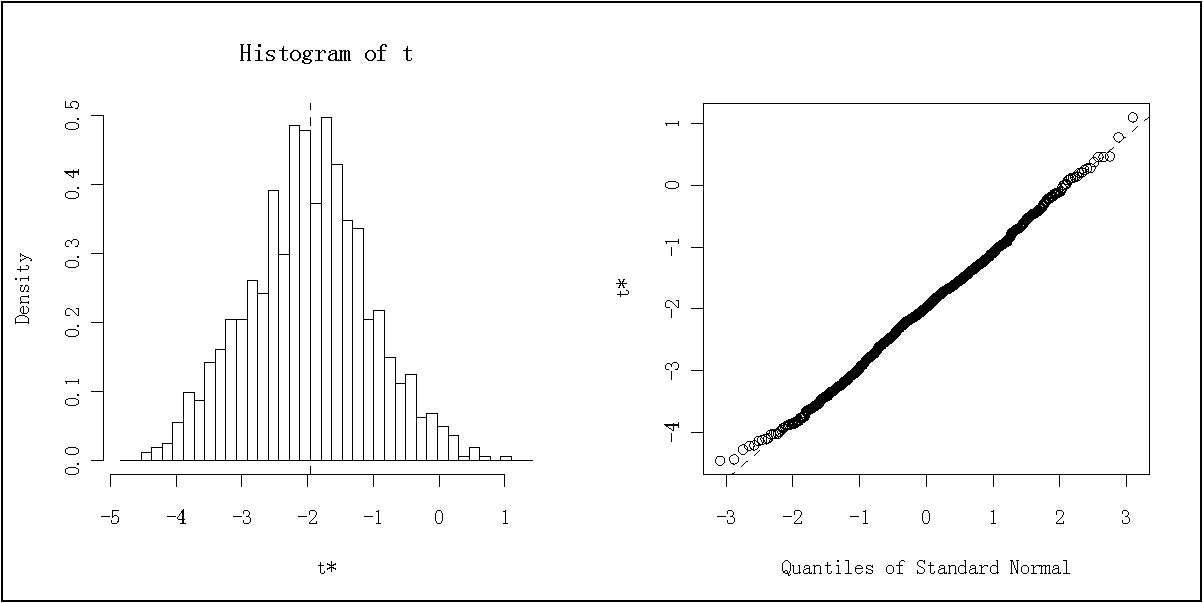
\includegraphics[width=0.6\textwidth]{chapter4-bootstrap-p3df-mean.pdf}
\end{center}
\caption{非专业与专业驾驶人最大舒适减速度$b_{max}$参数差值分层Bootstrap分布及正态Q-Q}
\label{p3-df-qq}
\end{figure}








%
%free us from the tedious assumptions
%bca confidence interval

%permutation test
%requirements



\section{本章小结}
本章通过对所采集数据进行处理和分析,研究了驾驶人行为特性的异同,发现非专业组和专业组驾驶人在自由行驶与跟驰的临界点,期望速度和最大减速度方面存在差异,为下一章研究驾驶人行为特性对交通流影响提供了依据。
